%%aQGC binned sig studies

\subsection{Initial study of the aQGC search strategy}

The aQGC terms can modify the amplitude of the VBS process at the higher effective center-of-mass energy, 
$m_{VV}$, as shown in Figure~\ref{fig:2lepaQGCshapeMVV}, hence merged regions are more important to enhance the signals.
Some studies below are based on Merged HP SR only.
It is found that the reconstructed $m_{VV}$ (or \mt\ in \zlep\ channel) is the best variable to separate the aQGC signals from the background,
while the RNN score distributions for the aQGC samples are similar to the one for the SM electroweak signal and still useful to suppress the non-VBS background as shown in Fig.~\ref{fig:2lepaQGCshapeRNN}.
Two-dimensional binning of $m_{VV}$ and the RNN score is used as the final discriminant for the aQGC search.
In this section, the optimal binning strategy is studied in \tlep\ channel.

\begin{figure}[]
    \centering
   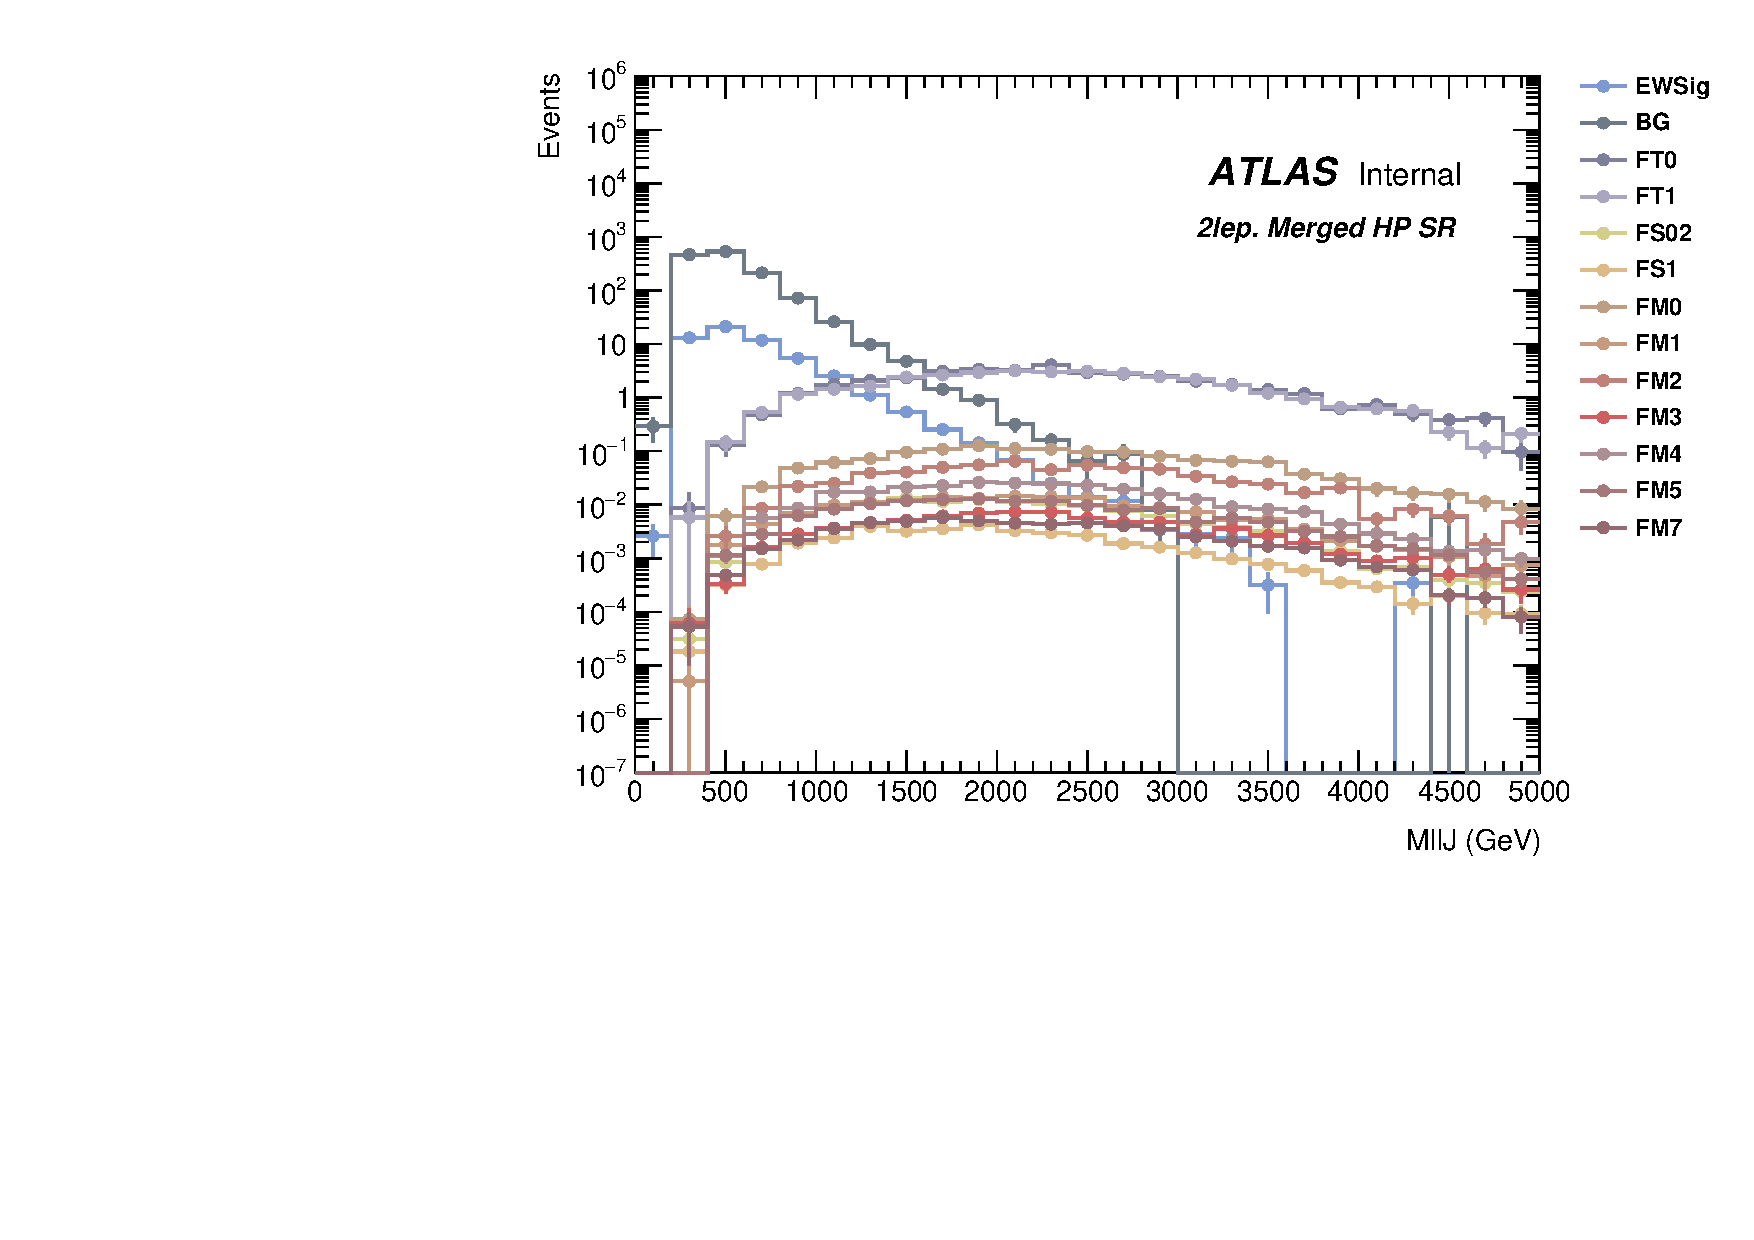
\includegraphics[width=0.45\textwidth]{figures/aQGC/MllJ_SR_HP_aQGC.pdf}
   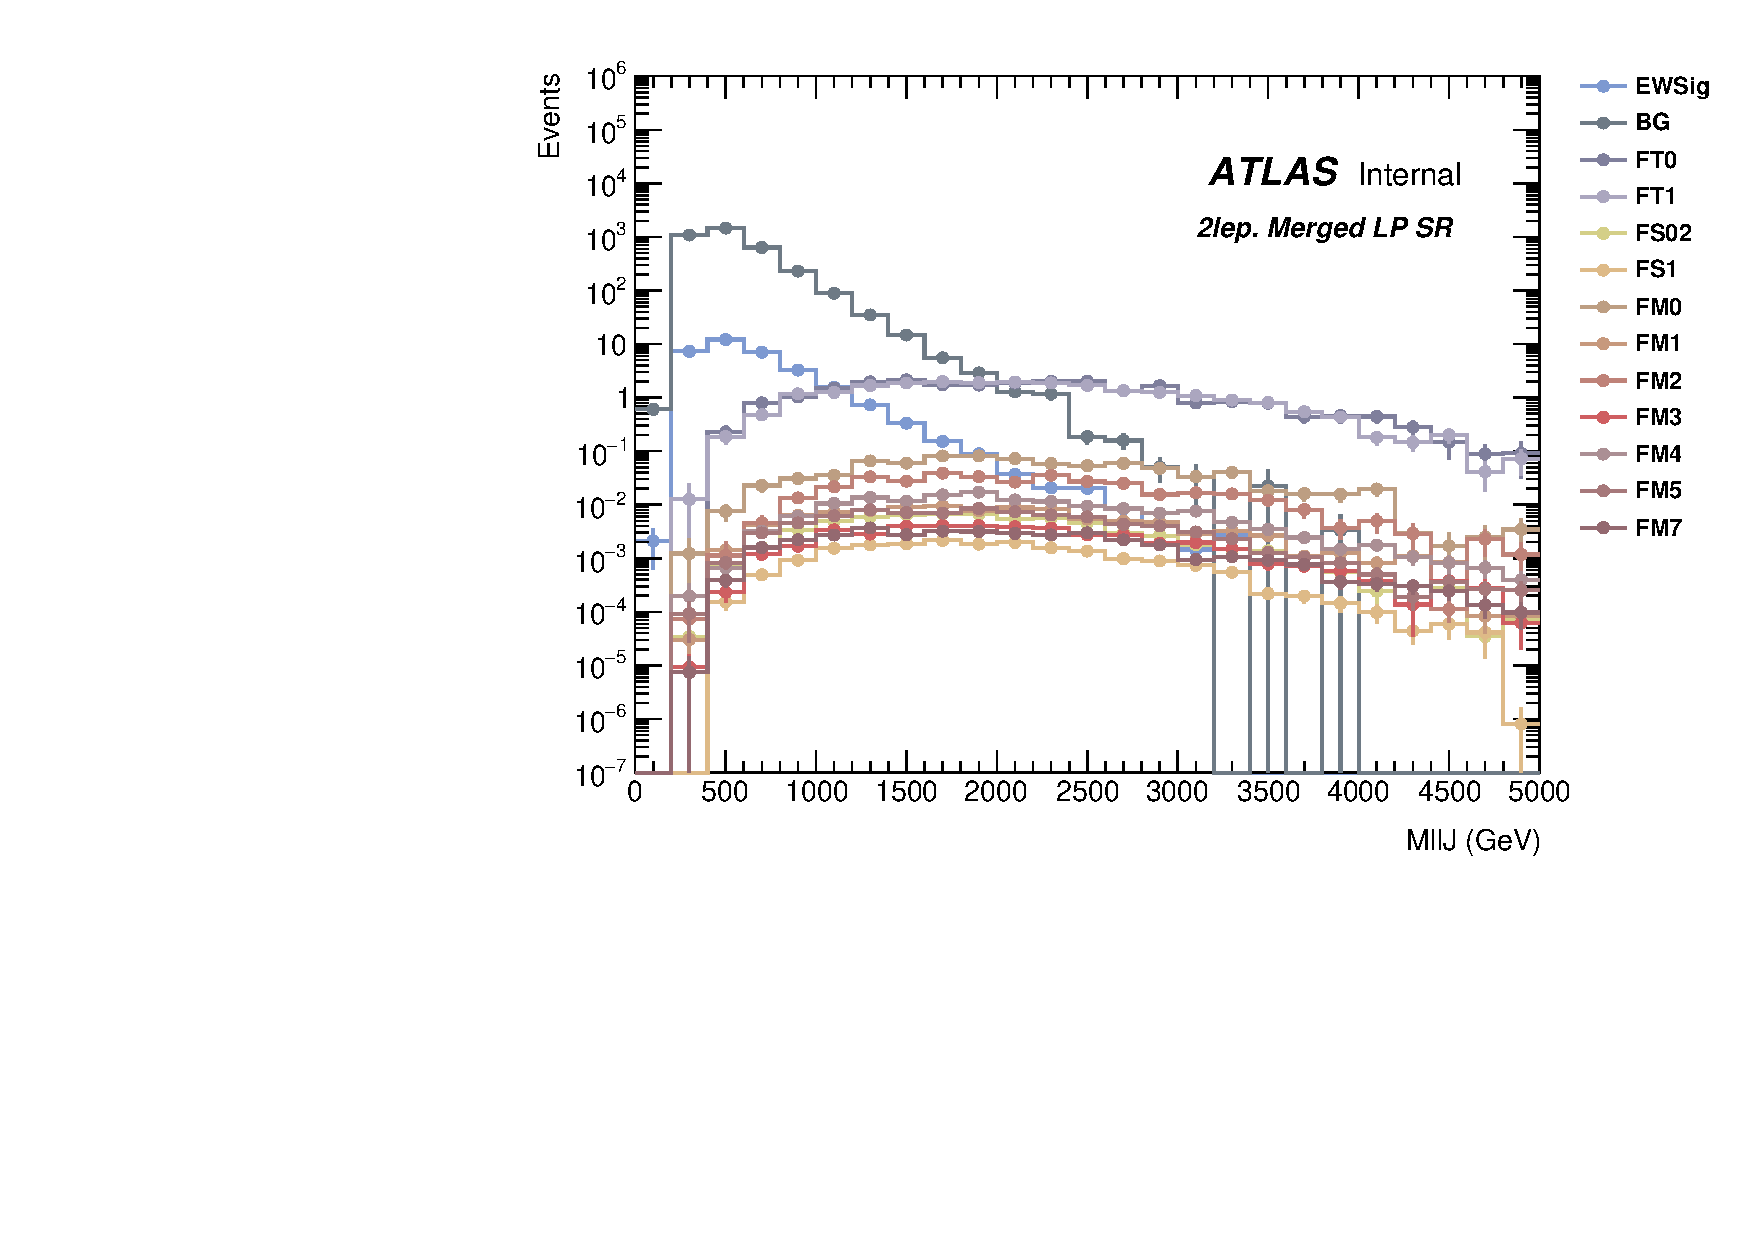
\includegraphics[width=0.45\textwidth]{figures/aQGC/MllJ_SR_LP_aQGC.pdf}
    \caption{$m_{VV}$ shape distribution of each wilson coefficient in Merged Signal regions. Only quadratic terms are shown.}
    \label{fig:2lepaQGCshapeMVV}
\end{figure}

\begin{figure}[]
    \centering
   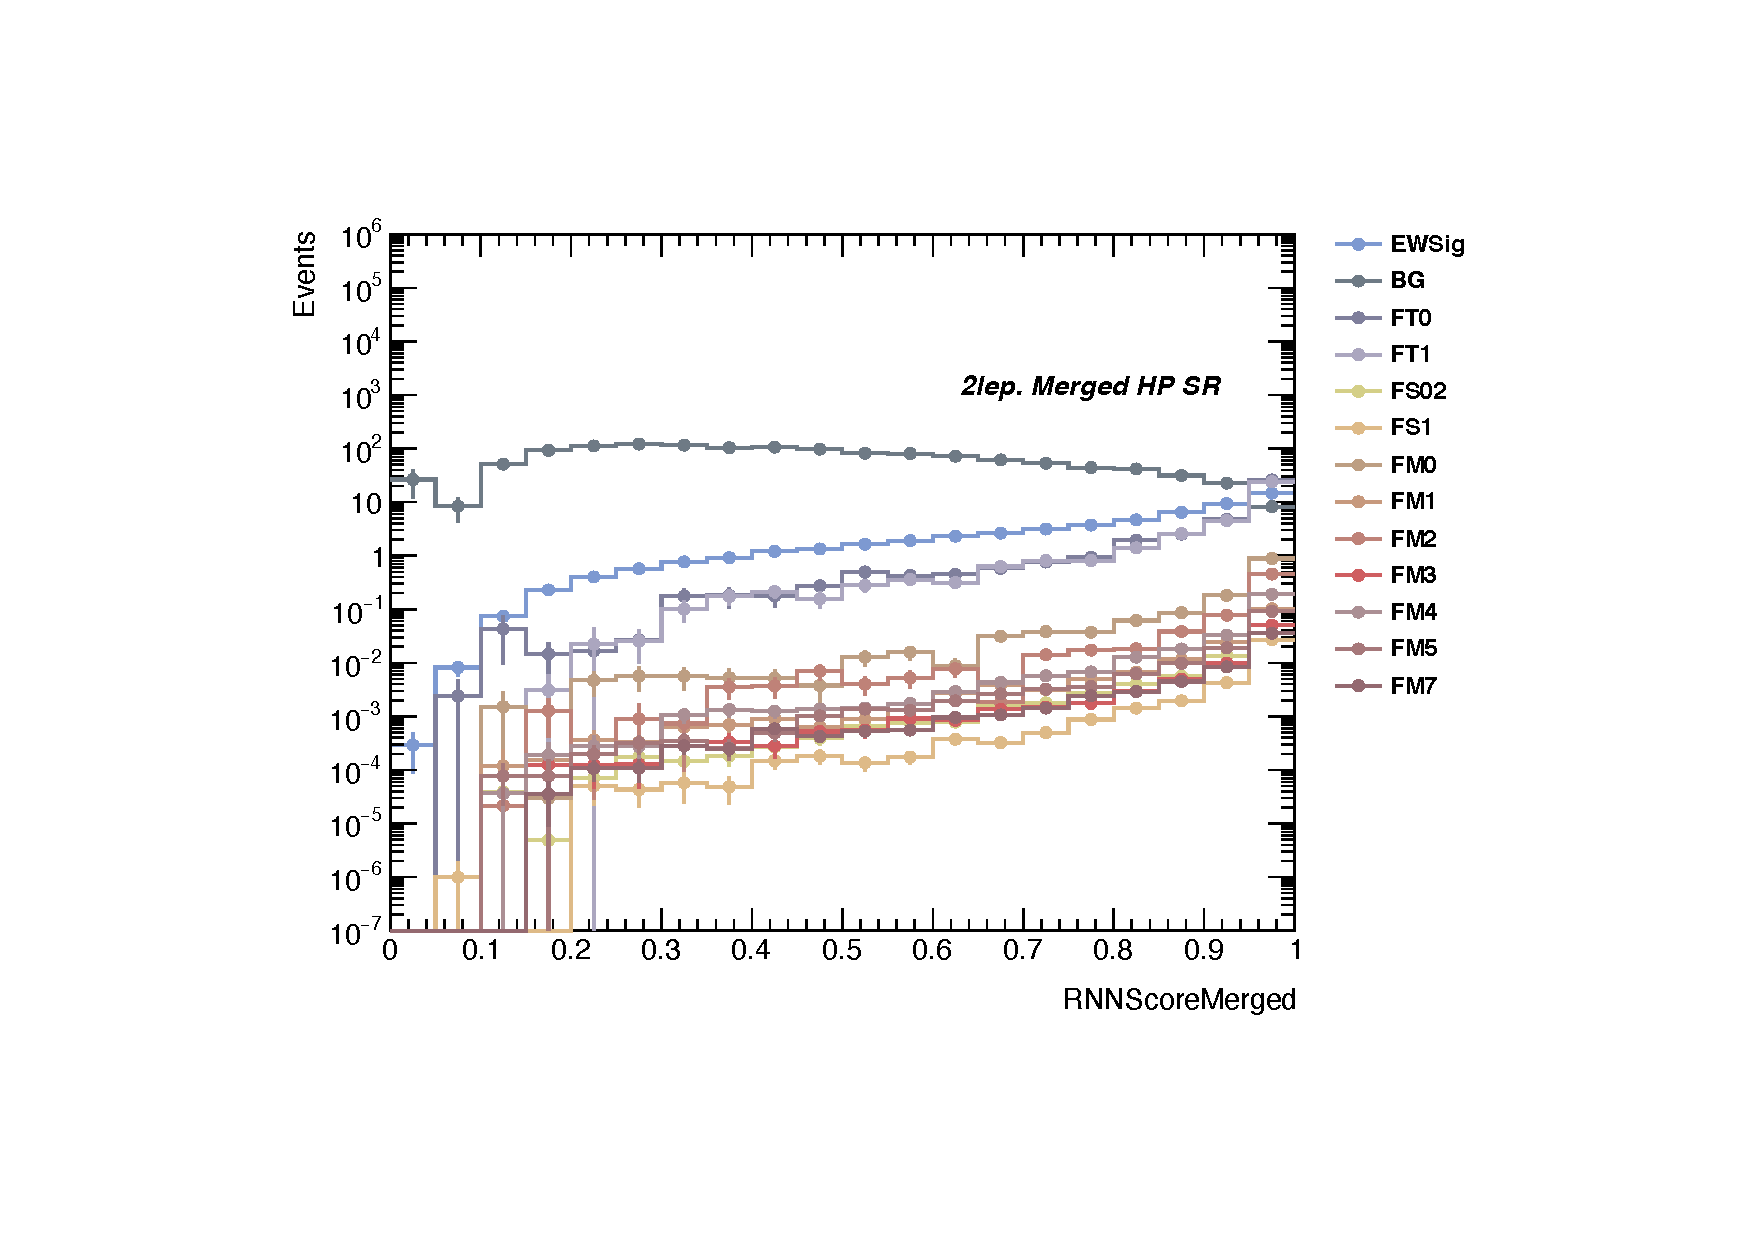
\includegraphics[width=0.45\textwidth]{figures/aQGC/RNNScoreMerged_SR_HP_aQGC.pdf}
   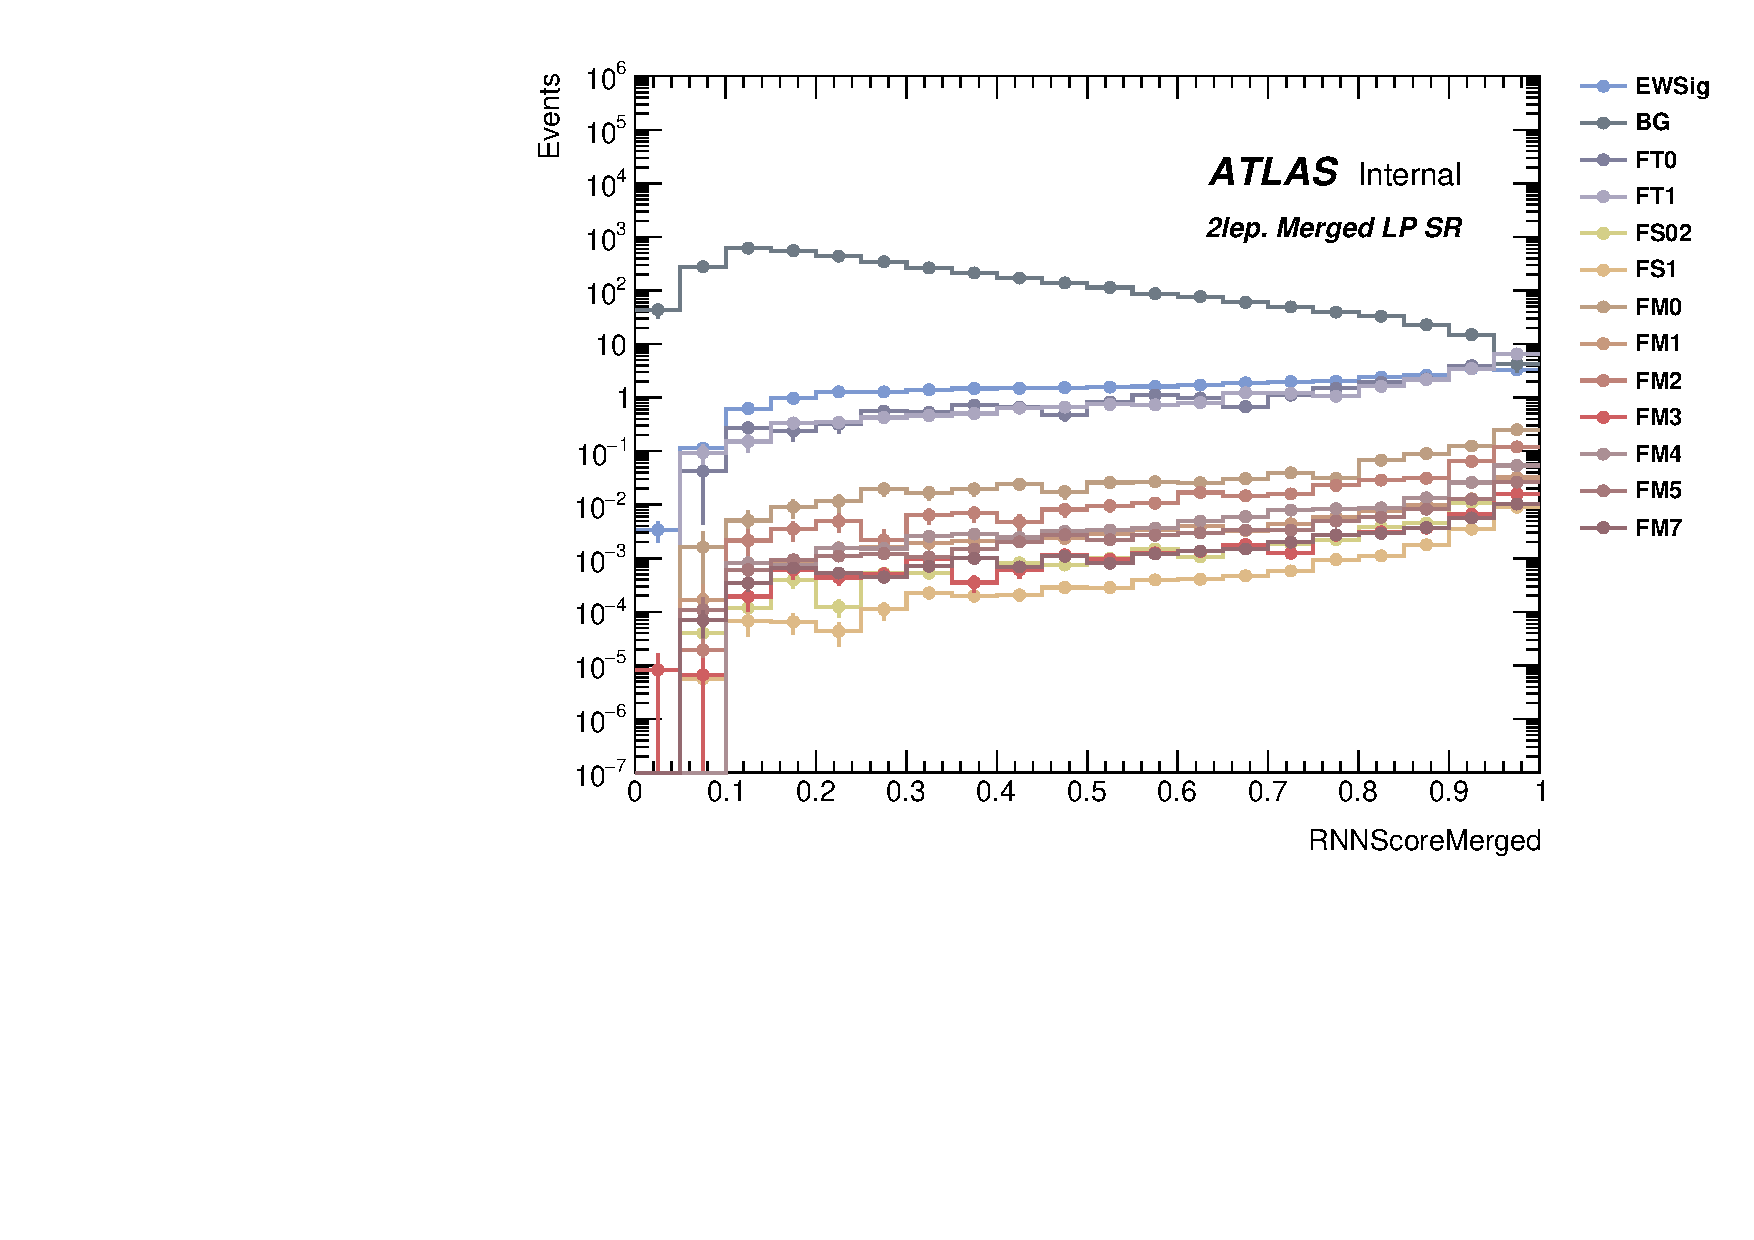
\includegraphics[width=0.45\textwidth]{figures/aQGC/RNNScoreMerged_SR_LP_aQGC.pdf}
    \caption{RNN score shape distribution of each wilson coefficient in Merged Signal regions. Only quadratic terms are shown.}
    \label{fig:2lepaQGCshapeRNN}
\end{figure}

The binned significance defined as:
%
\begin{eqnarray*}
  Z = \sqrt{\sum_{bins}\left[2(s + b)ln\left(\frac{(s + b)(b+\sigma^2_{b})}{b^2+(s+b)\sigma^2_{b}}\right) - \frac{b^2}{\sigma^2_{b}}ln\left(1+\frac{\sigma^2_{b}s}{b(b+\sigma^2_{b})}\right)\right]} \\
\end{eqnarray*}
%
is used in this study.
The $s$ is the number of the aQGC signal for the given wilson coefficient.
Signal samples are normalized to $\frac{f_{i}}{\Lambda^4}=1.0$ and no clipping energy requirement described in Section~\ref{subsec:clipping} is applied. Only the quadratic term is used in this study since the interference term is negligibly small with this parameter choice.
The $b$ includes the SM electroweak signals and the other backgrounds (like $Z$+jets, \ttbar, QCD diboson).
The fractional systematic uncertainty $\sigma_{b} = 0.2$ is assumed.

For simplicity, and the background estimation stability by keeping the number of bins as small as possible, two different approaches are tested.
One is to use the $m_{VV}$ distribution for the binned significance definition, after the certain cut on the RNN score to suppress the SM background.
The other is to use the RNN score distribution for the binned significance calculation, after the cut on the $m_{VV}$ to enhance the aQGC signals.
We also varied the threshold for $\mathrm{M}_{tagjj}$ at the same time.

Figure~\ref{fig:2lepaQGCBinnedSigMVV} shows the binned significance calculated by using $m_{VV}$ distribution after the cuts on RNN score and $\mathrm{M}_{tagjj}$, as functions of the varied thresholds of them.
It is found a cut on RNN score does not help to improve the sensitivity so much,
and a cut on $\mathrm{M}_{tagjj}$ deteriorates it.
On the other hand, Figure~\ref{fig:2lepaQGCBinnedSigRNN} shows the binned significance by using RNN score distribution
after the cuts on $m_{VV}$ and $\mathrm{M}_{tagjj}$, as functions of the thresholds for them.
The result depends on the threshold for $m_{VV}$, depending on the signal strength (under the $f_i/\Lambda^4 = 1.0$ constraint, $f_{S}$ signals have smaller signal yields than $f_{T}$ and $f_{M}$ and tighter cut on $m_{VV}$ is preferred, but it is just a result of the arbitral choice).
The significance value for each wilson coefficient term is summarized in tables~\ref{tab:2lep_HPSR_MVV} to \ref{tab:2lep_LPSR_RNN}.
Generally, about 5--10\% better sensitivity can be obtained by using RNN score distribution after the cut on $m_{VV}$ at the certain threshold.

\begin{figure}[ht]
    \centering
    	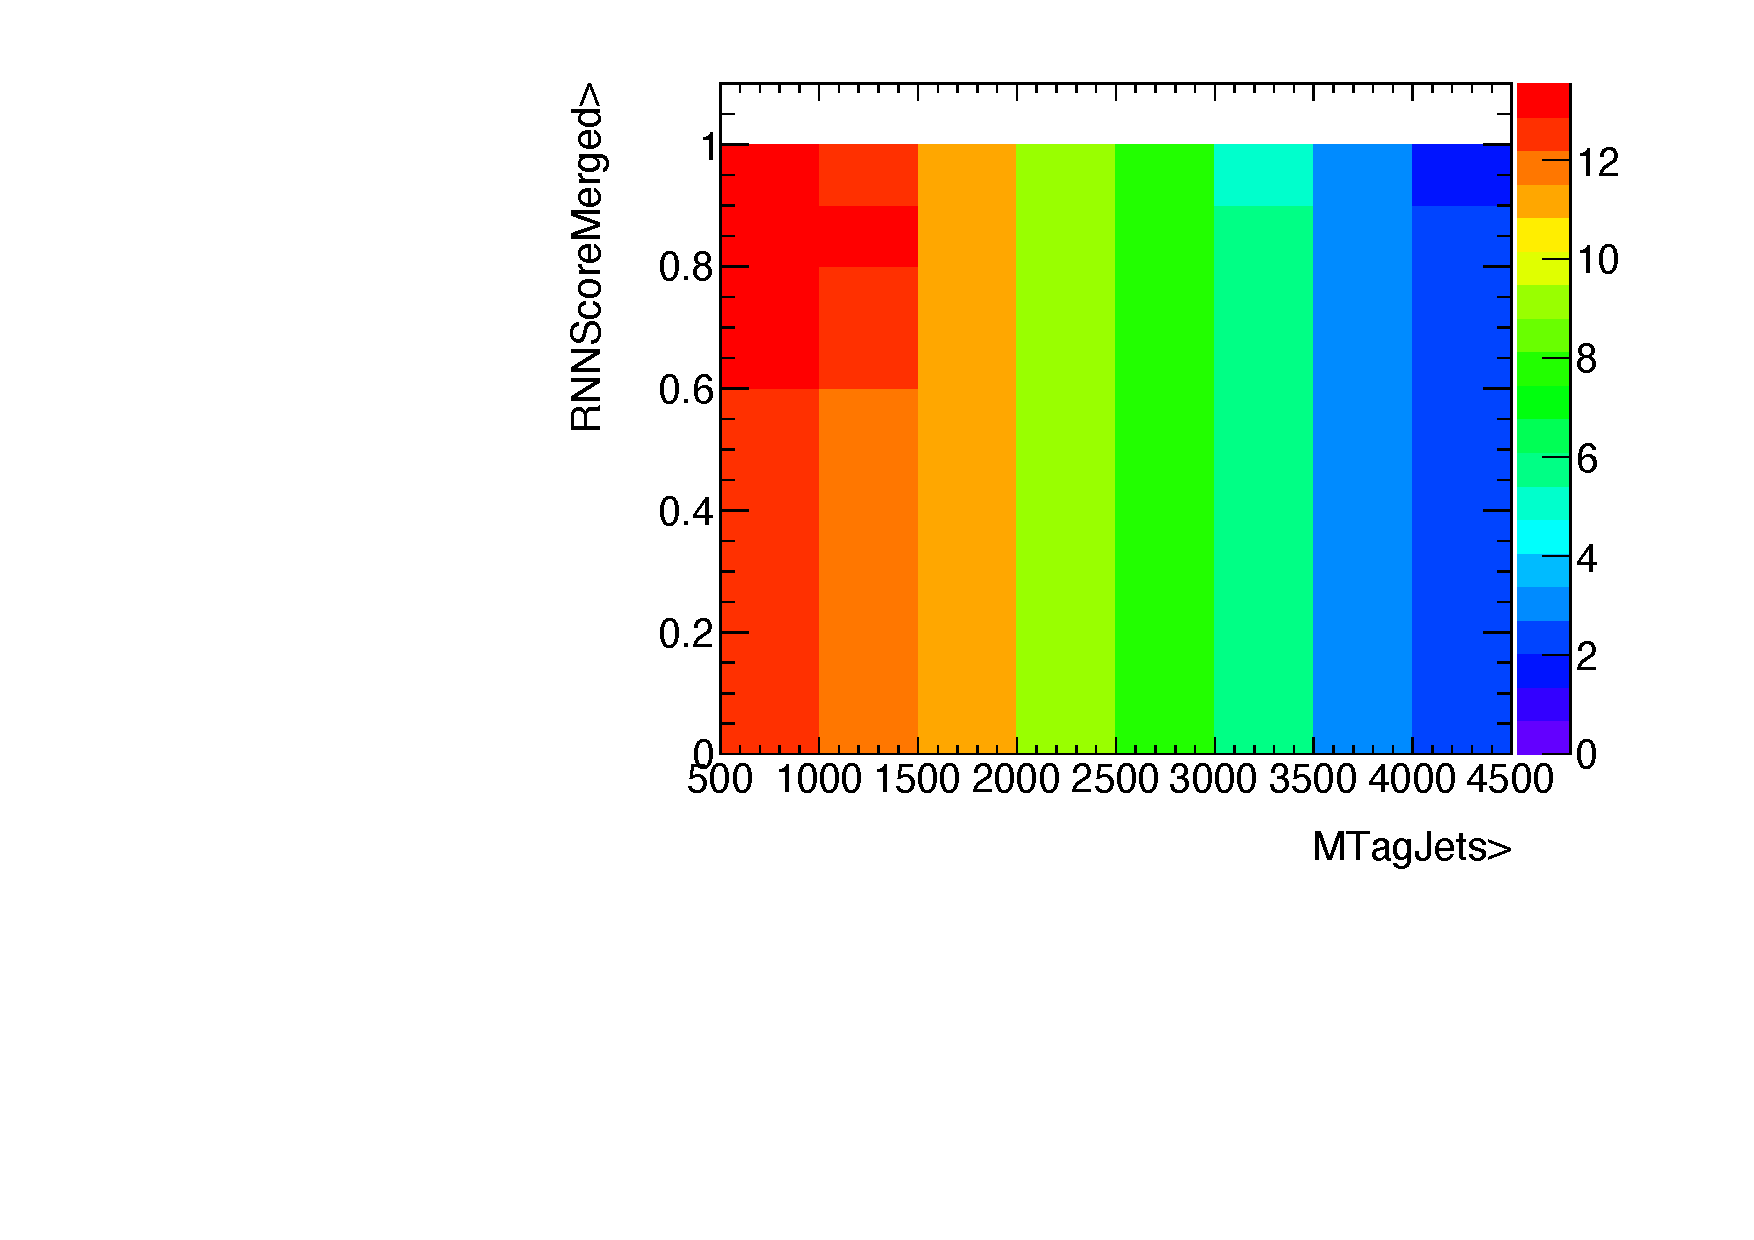
\includegraphics[width=0.30\textwidth]{figures/aQGC/HPSRFT0MVV.pdf}
    	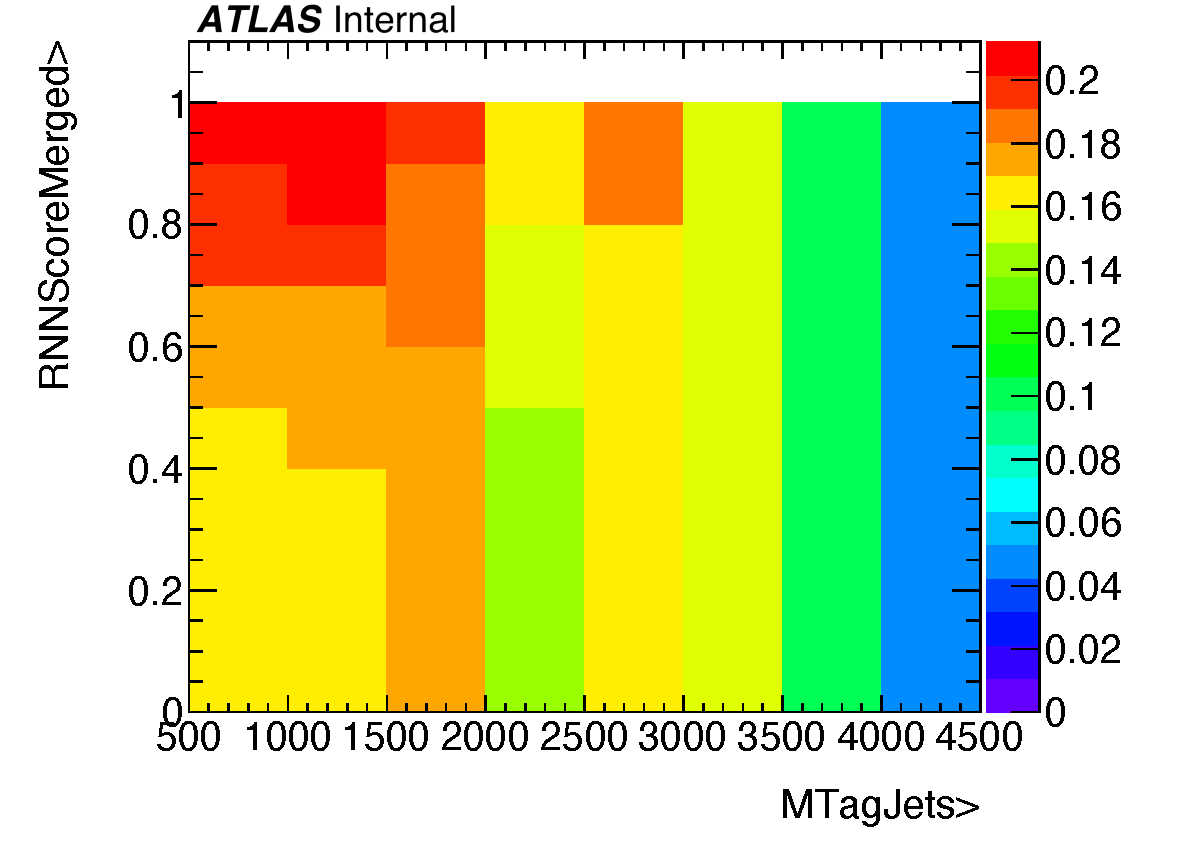
\includegraphics[width=0.30\textwidth]{figures/aQGC/HPSRFS02MVV.pdf}
        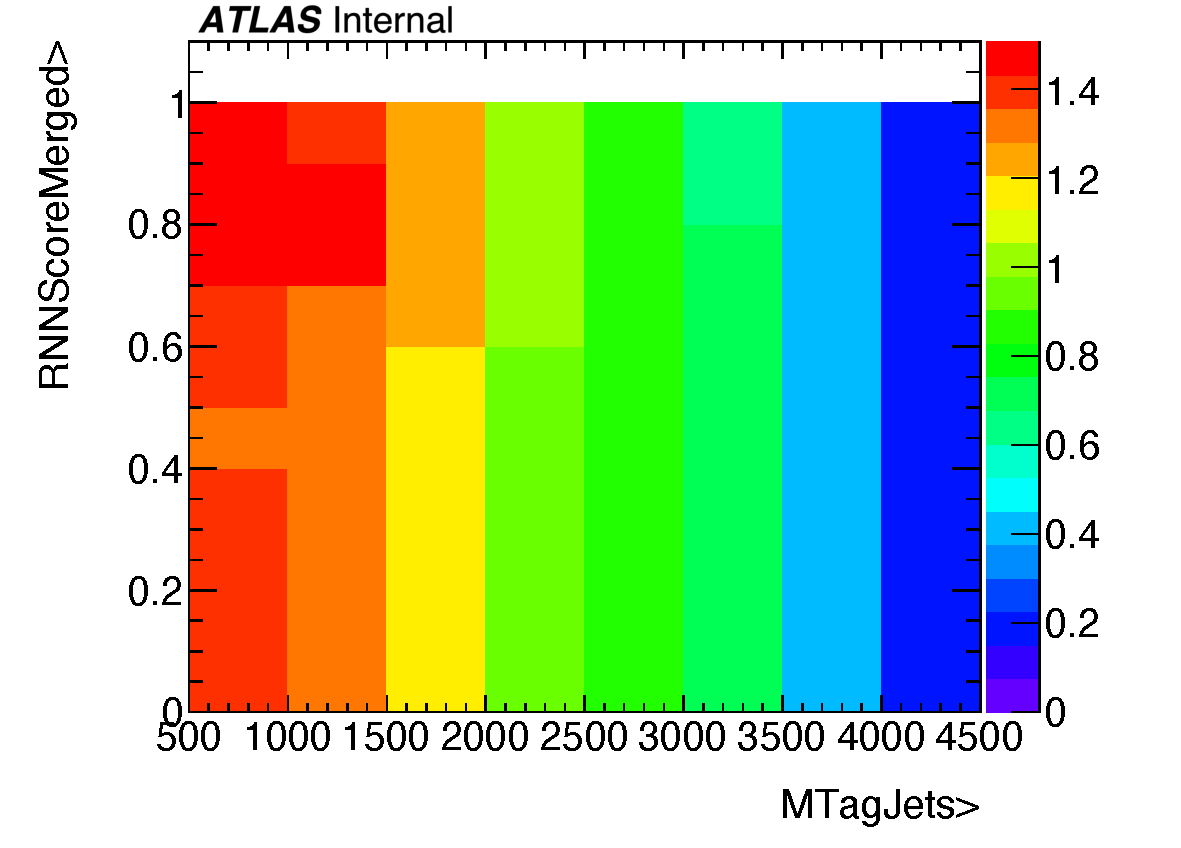
\includegraphics[width=0.30\textwidth]{figures/aQGC/HPSRFM0MVV.pdf}
        \caption{The 2D scan of the binned significance of operator FT0 (left), FS02 (middle), FM0 (right) with $m_{VV}$ score as discriminant in Merged HP signal region. Only quadratic terms are scanned.}
        \label{fig:2lepaQGCBinnedSigMVV}
\end{figure}

\begin{figure}[ht]
    \centering
    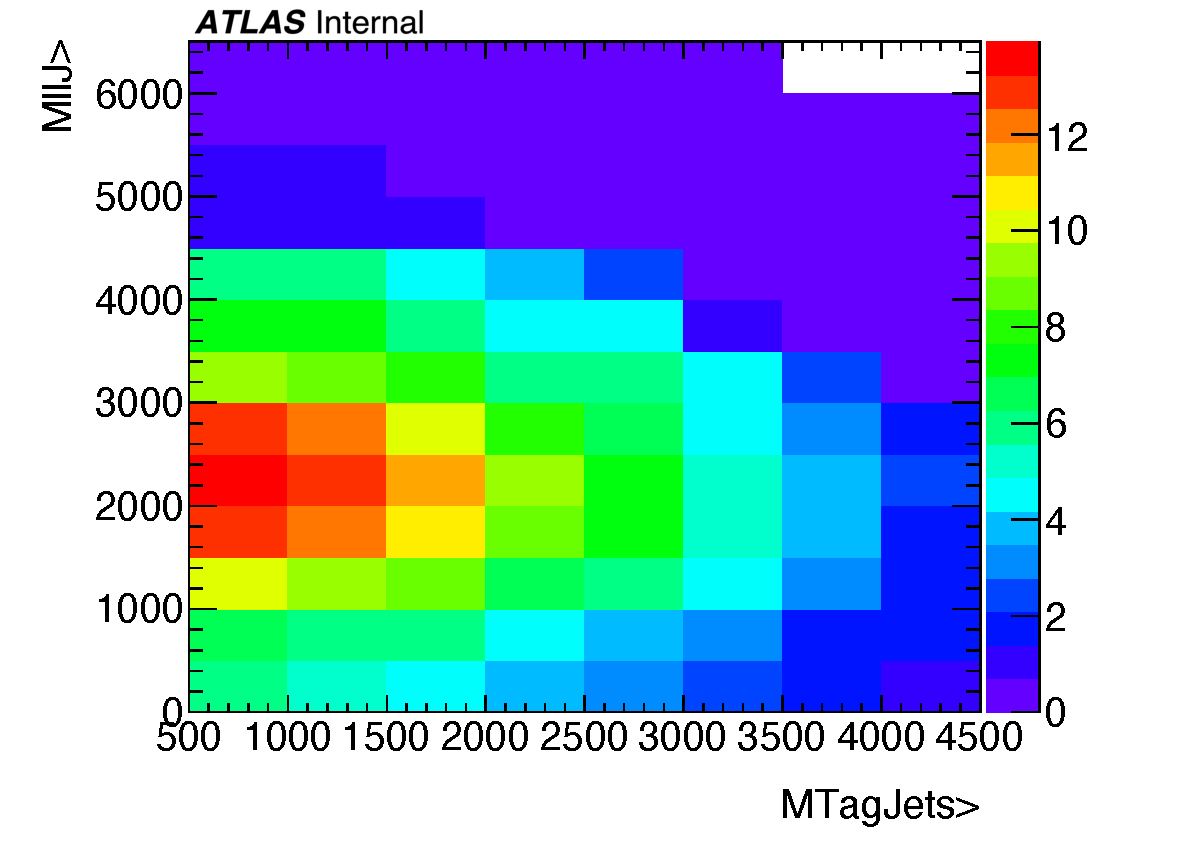
\includegraphics[width=0.30\textwidth]{figures/aQGC/HPSRFT0RNN.pdf}
    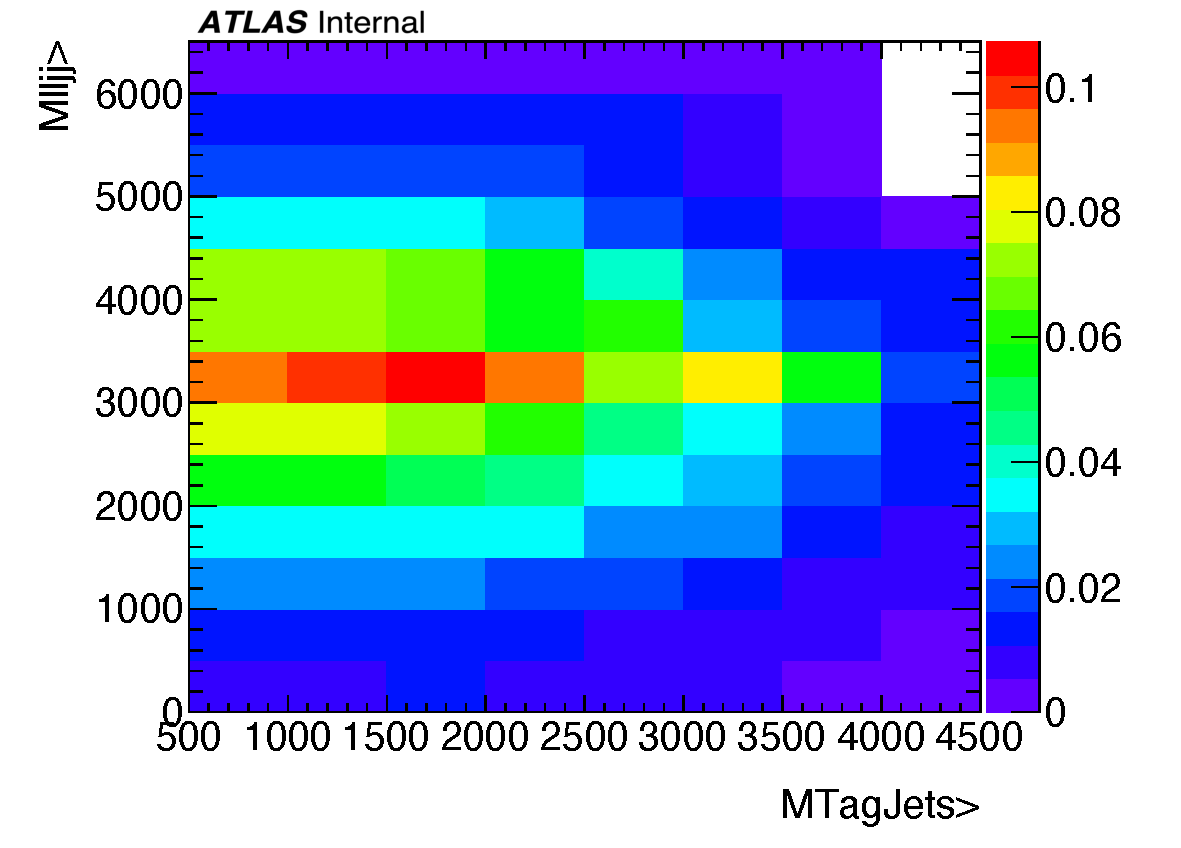
\includegraphics[width=0.30\textwidth]{figures/aQGC/HPSRFS02RNN.pdf}
  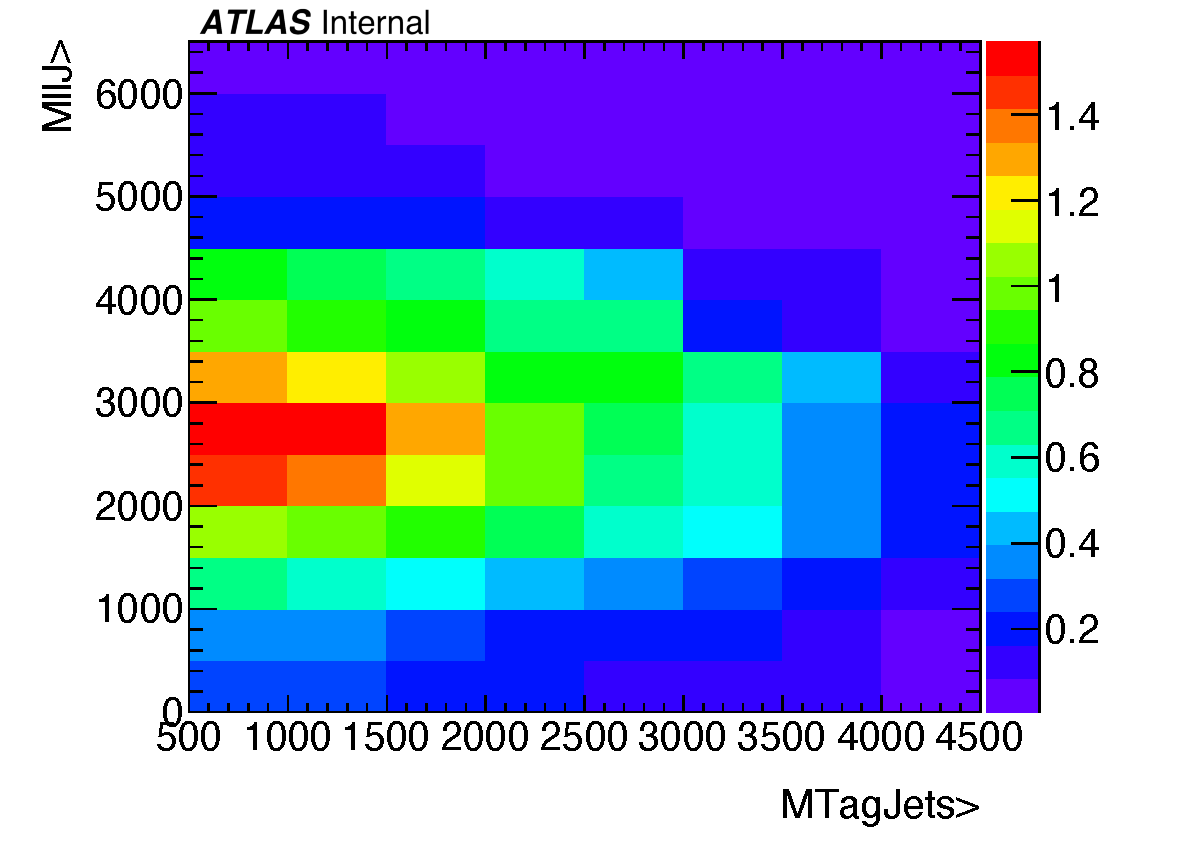
\includegraphics[width=0.30\textwidth]{figures/aQGC/HPSRFM0RNN.pdf}
        \caption{The 2D scan of the binned significance of operator FT0 (left), FS02 (middle), FM0 (right) with RNN score as discriminant in Merged HP signal region. Only quadratic terms are scanned.}
        \label{fig:2lepaQGCBinnedSigRNN}
\end{figure}

\begin{table}[ht!]
\small
\begin{center}
\resizebox{0.50\textwidth}{!}{

 \begin{tabular}{ r ||  r  r  r  r  |}
    & $\mathrm{M}_{tagjj}$ (GeV) & RNN score  & significance before cut& significance  \tabularnewline \hline
FT0 & 500                        & 0.6        & 12.55                  & 12.98         \tabularnewline \hline
FT1 & 500                        & 0.6        & 11.94                  & 12.50         \tabularnewline \hline
FS02& 1000                       & 0.8        & 0.17                   & 0.20          \tabularnewline \hline
FS1 & 500                        & 0.8        & 0.07                   & 0.07          \tabularnewline \hline
FM0 & 500                        & 0.7        & 1.36                   & 1.50          \tabularnewline \hline
FM1 & 500                        & 0.3        & 0.25                   & 0.27          \tabularnewline \hline
FM2 & 500                        & 0.7        & 0.82                   & 0.93          \tabularnewline \hline
FM3 & 500                        & 0.6        & 0.15                   & 0.16          \tabularnewline \hline
FM4 & 500                        & 0.7        & 0.38                   & 0.42          \tabularnewline \hline
FM5 & 500                        & 0.7        & 0.23                   & 0.25          \tabularnewline \hline
FM7 & 500                        & 0.6        & 0.12                   & 0.12          \tabularnewline \hline

\end{tabular}
}
\caption{Best cut point table for binned significance for $m_{VV}$ score distribution in \tlep channel in HPSR}
\label{tab:2lep_HPSR_MVV}
\end{center}
\end{table}

\begin{table}[ht!]
\small
\begin{center}
\resizebox{0.50\textwidth}{!}{

 \begin{tabular}{ r ||  r  r  r  r  |}
    & $\mathrm{M}_{tagjj}$ (GeV) & RNN score  & significance before cut & significance \tabularnewline \hline
FT0 & 500          & 0.1  & 6.65      & 6.77                          \tabularnewline \hline
FT1 & 500          & 0.2  & 6.69      & 6.85                          \tabularnewline \hline
FS02& 500          & 0.9  & 0.05      & 0.10                          \tabularnewline \hline
FS1 & 1000         & 0.8  & 0.02      & 0.04                          \tabularnewline \hline
FM0 & 500          & 0.8  & 0.54      & 0.12                          \tabularnewline \hline
FM1 & 500          & 0.1  & 0.08      & 0.42                          \tabularnewline \hline
FM2 & 500          & 0.9  & 0.28      & 0.08                          \tabularnewline \hline
FM3 & 1000         & 0.8  & 0.05      & 0.18                          \tabularnewline \hline
FM4 & 1000         & 0.8  & 0.12      & 0.10                          \tabularnewline \hline
FM5 & 1000         & 0.8  & 0.07      & 0.10                          \tabularnewline \hline
FM7 & 500          & 0.1  & 0.04      & 0.06                          \tabularnewline \hline

\end{tabular}
}
\caption{Best cut point table for binned significance for $m_{VV}$ score distribution in \tlep channel in LPSR}
\label{tab:2lep_LPSR_MVV}
\end{center}
\end{table}

\begin{table}[ht!]
\small
\begin{center}
\resizebox{0.50\textwidth}{!}{

 \begin{tabular}{ r ||  r  r  r  r  |}
    & $\mathrm{M}_{tagjj}$ (GeV) & MllJ (GeV) & significance before cut& significance \tabularnewline \hline
FT0 & 500          & 2000   & 5.62    & 13.92                           \tabularnewline \hline
FT1 & 500          & 2000   & 5.25    & 13.31                           \tabularnewline \hline
FS02& 1500         & 3000   & 0.01    & 0.11                            \tabularnewline \hline
FS1 & 2500         & 3000   & 0.01    & 0.07                            \tabularnewline \hline
FM0 & 500          & 2500   & 0.27    & 1.57                            \tabularnewline \hline
FM1 & 500          & 2500   & 0.03    & 0.28                            \tabularnewline \hline
FM2 & 500          & 2500   & 0.14    & 0.95                            \tabularnewline \hline
FM3 & 500          & 3000   & 0.01    & 0.12                            \tabularnewline \hline
FM4 & 500          & 2500   & 0.06    & 0.45                            \tabularnewline \hline
FM5 & 500          & 2500   & 0.03    & 0.25                            \tabularnewline \hline
FM7 & 500          & 2500   & 0.01    & 0.12                            \tabularnewline \hline

\end{tabular}
}
\caption{Best cut point table for binned significance for RNN score distribution in \tlep channel in HPSR}
\label{tab:2lep_HPSR_RNN}
\end{center}
\end{table}

\begin{table}[ht!]
\small
\begin{center}
\resizebox{0.50\textwidth}{!}{

 \begin{tabular}{ r ||  r  r  r  r  |}
    & $\mathrm{M}_{tagjj}$ (GeV) & MllJ (GeV) & significance before cut& significance \tabularnewline \hline
FT0 & 500          & 2000  & 2.64     & 7.72                            \tabularnewline \hline
FT1 & 500          & 2000  & 2.80     & 7.46                            \tabularnewline \hline
FS02& 1500         & 3000  & 0.01     & 0.06                            \tabularnewline \hline
FS1 & 500          & 3000  & 0.00     & 0.06                            \tabularnewline \hline
FM0 & 500          & 2500  & 0.12     & 0.92                            \tabularnewline \hline
FM1 & 500          & 3000  & 0.02     & 0.18                            \tabularnewline \hline
FM2 & 500          & 3000  & 0.06     & 0.54                            \tabularnewline \hline
FM3 & 500          & 3000  & 0.01     & 0.12                            \tabularnewline \hline
FM4 & 500          & 3000  & 0.03     & 0.26                            \tabularnewline \hline
FM5 & 500          & 3000  & 0.01     & 0.16                            \tabularnewline \hline
FM7 & 500          & 3000  & 0.01     & 0.09                            \tabularnewline \hline

\end{tabular}
}
\caption{Best cut point table for binned significance for RNN score distribution in \tlep channel LPSR}
\label{tab:2lep_LPSR_RNN}
\end{center}
\end{table}

Following the study of this section, a more reliable study based on the profile likelihood fit is performed
in Section~\ref{subsec:2binapproach}, using the RNN score as a discriminant after the cut on $m_{VV}$.
%\subsection{Expected limit}
%\label{subsec:aqgc_limit}

%The expected upper limit on each wilson coefficient by a combined fit of all 3 channels is shown in table~\ref{tab:aQGC_limit}, which is calculated by $\sqrt{\mu_{95\%}} = f_{i} / \Lambda^4$, where $\mu_{95\%}$ is the 95\% upper limit on the signal strength.
%The $m_{VV}$ distributions without any additional cuts are used in the fit.
%The systematic uncertainties are yet to be included.
%Figures~\ref{fig:0lepFT0} and ~\ref{fig:1lepFT0}, ~\ref{fig:2lepFT0} show the prefit plots of $m_{VV}$ distribution. FT0 signal is overlaid.

%\begin{table}[ht!]
%\small
%\begin{center}
%\resizebox{0.30\textwidth}{!}{
% \begin{tabular}{ | r || r |}
%    & Expected limit (TeV$^{-4})$ \tabularnewline \hline
%FT0 & 0.14                        \tabularnewline \hline
%FT1 & 0.14                        \tabularnewline \hline
%FS02& 2.90                        \tabularnewline \hline
%FS1 & 4.56e+6                     \tabularnewline \hline
%FM0 & 0.85                        \tabularnewline \hline
%FM1 & 2.55                        \tabularnewline \hline
%FM2 & 1.26                        \tabularnewline \hline
%FM3 & 4.69e+2                     \tabularnewline \hline
%FM4 & 2.07                        \tabularnewline \hline
%FM5 & 81.3                        \tabularnewline \hline
%FM7 & 5.37e+2                     \tabularnewline \hline
%\end{tabular}
%}
%\caption{Expected upper limits of each wilson coefficient. All 3 channels are combined.}
%\label{tab:aQGC_limit}
%\end{center}
%\end{table}
%
%\begin{figure}[ht]
%    \centering
%    	\subfigure[ 0lep merged CR ]{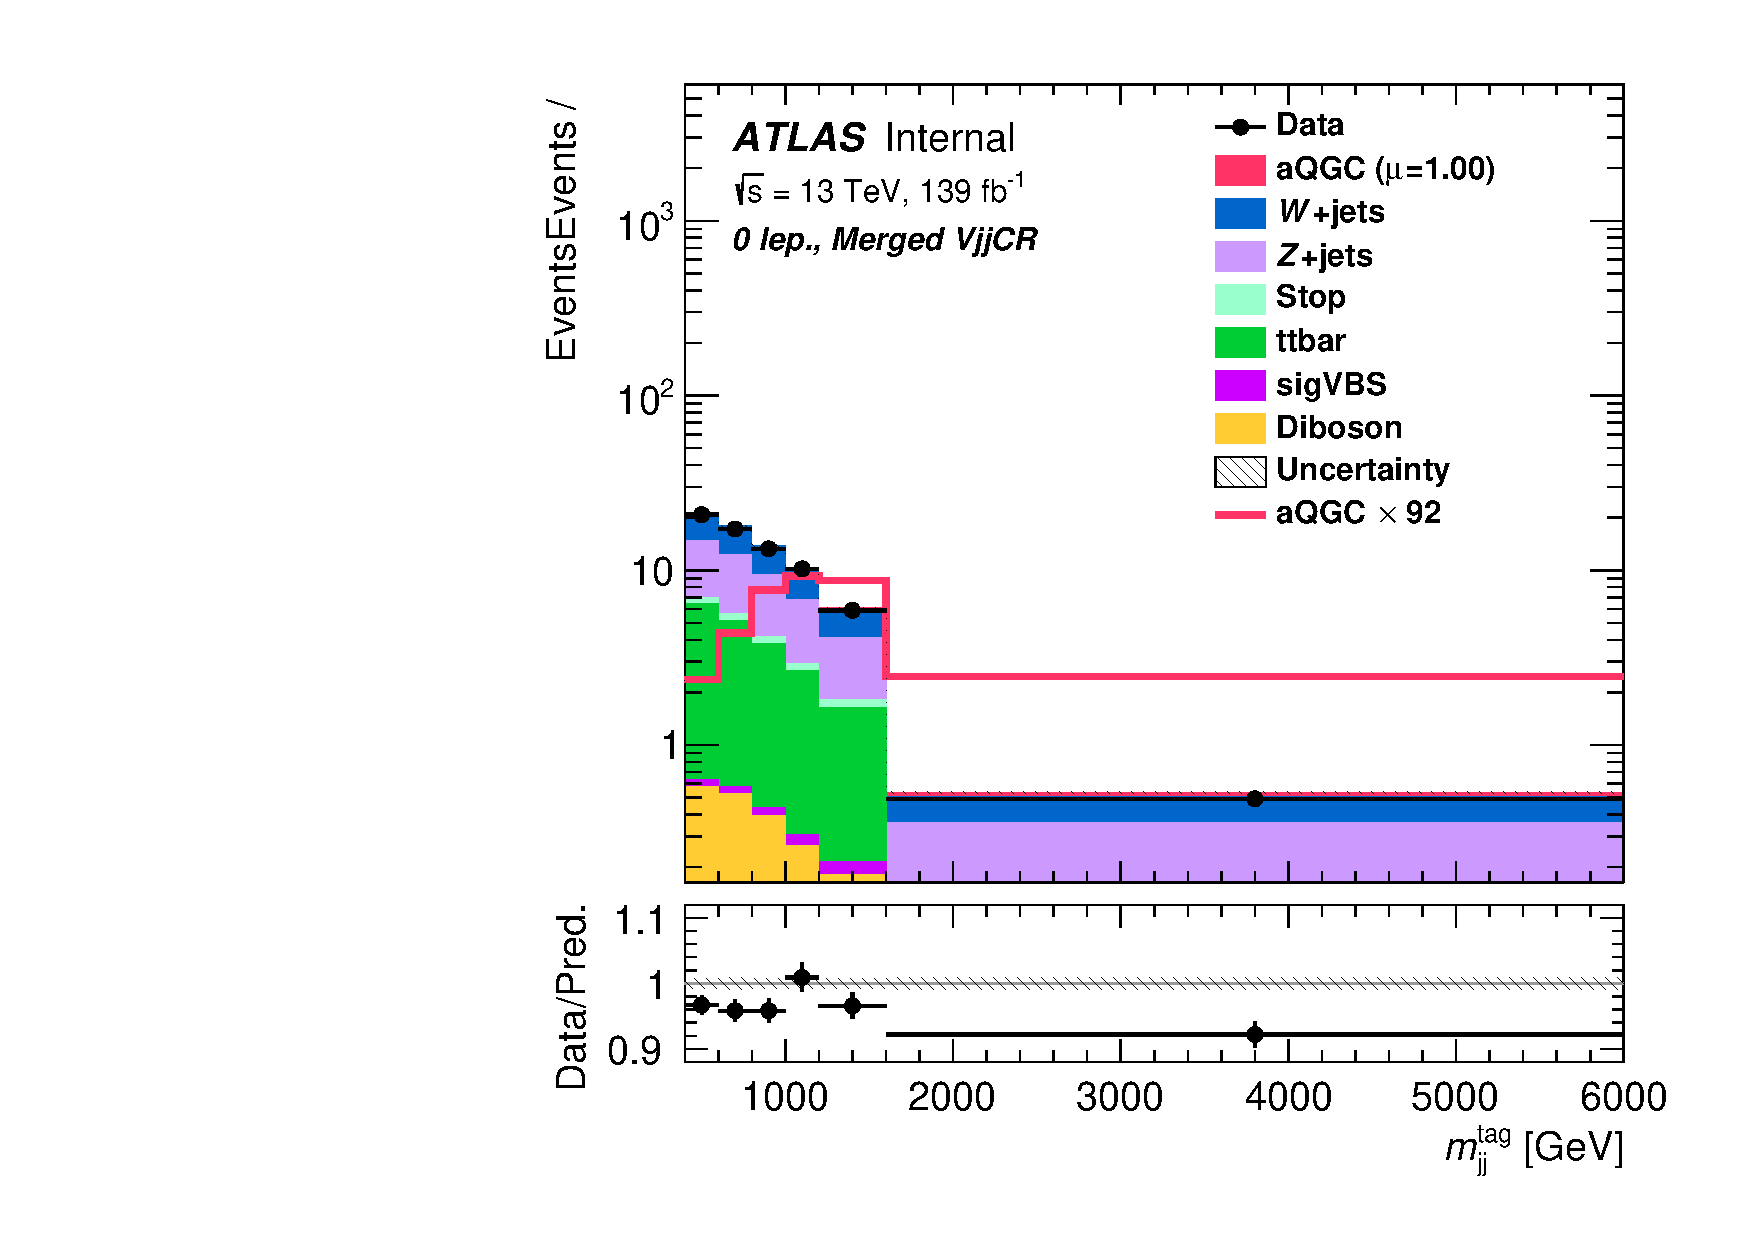
\includegraphics[width=0.32\textwidth]{figures/aQGC/Region_distMTagJets_DCRVjetMer_BMin0_J0_incJet1_L0_T0_incFat1_Y6051_incTag1_Fat1_Prefitlog.pdf}}
%    	\subfigure[ 0lep HP SR ]{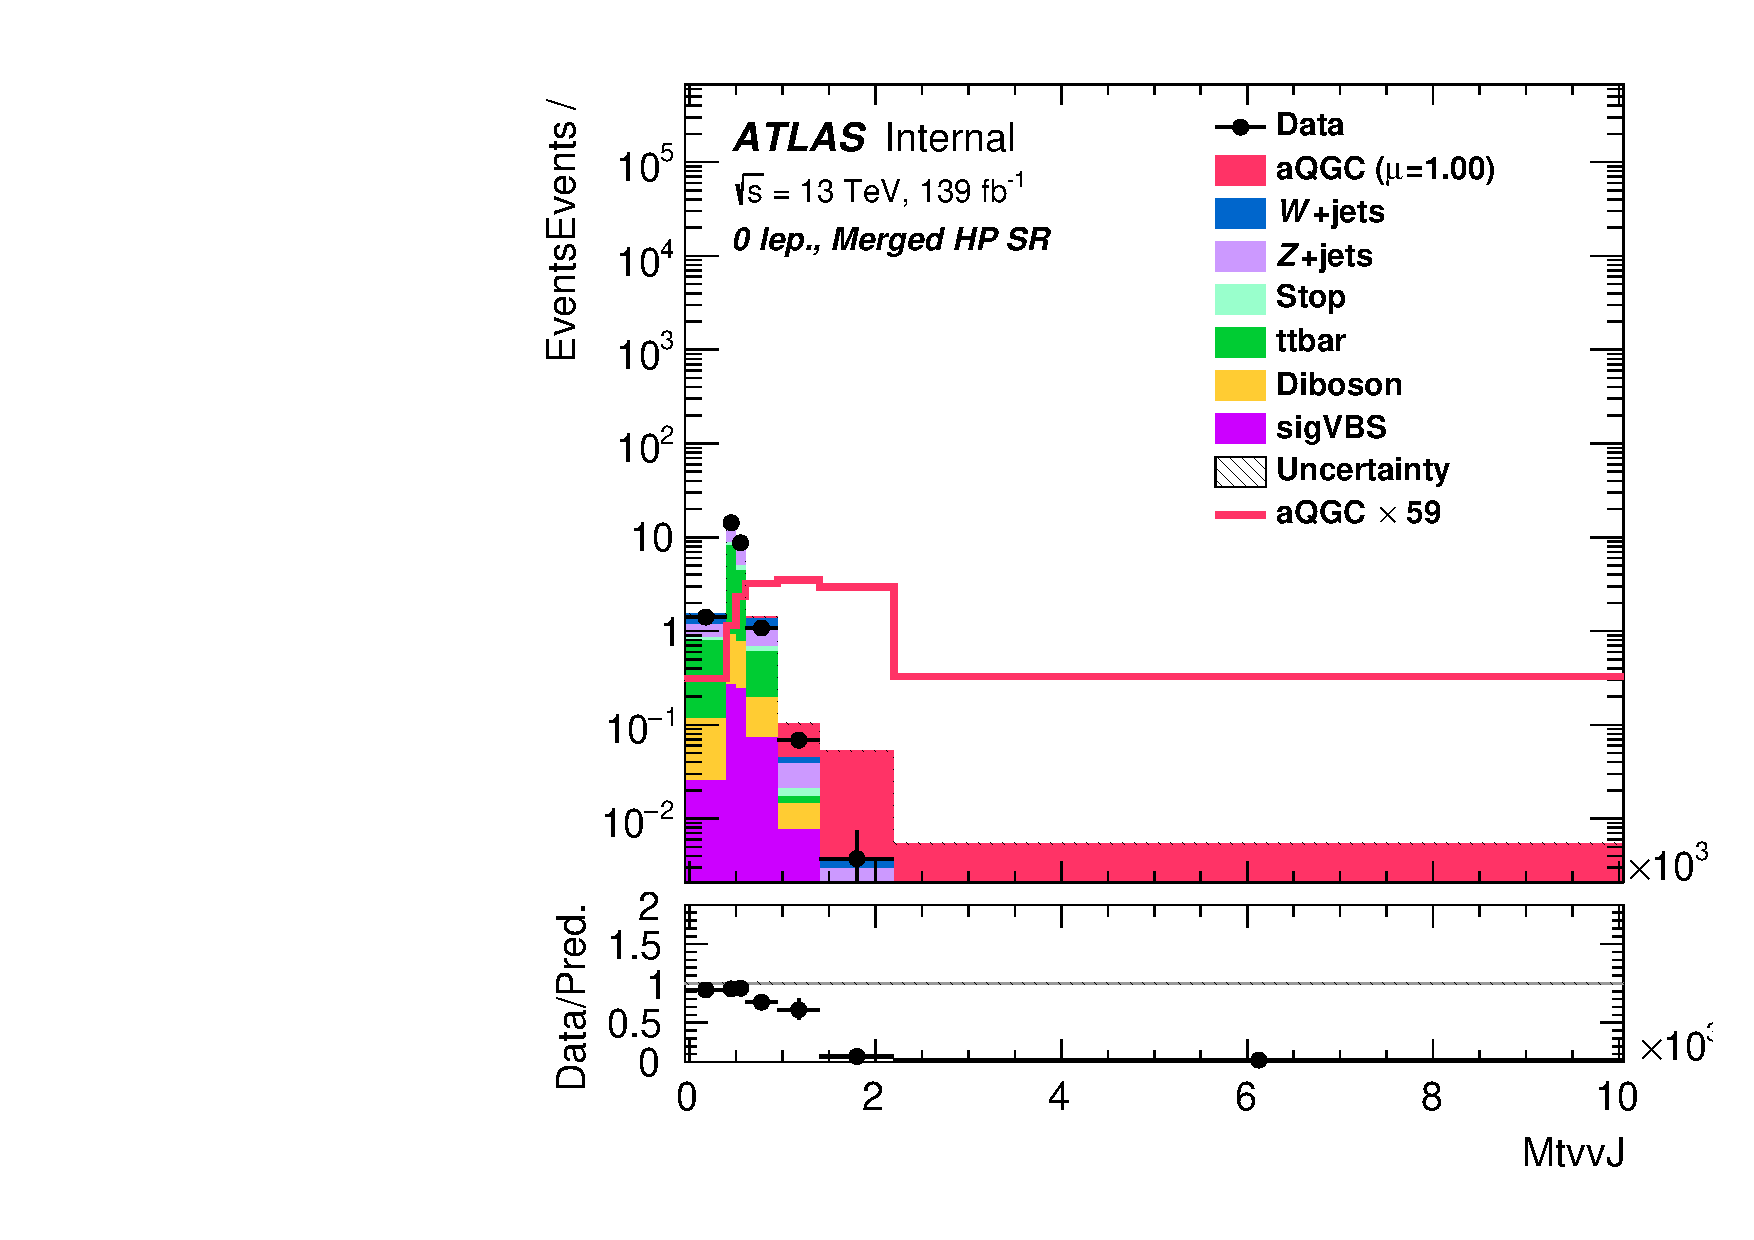
\includegraphics[width=0.32\textwidth]{figures/aQGC/Region_distMtvvJ_DSRVBSHP_BMin0_J0_incJet1_L0_T0_incFat1_Y6051_incTag1_Fat1_Prefitlog.pdf}}
%    	\subfigure[ 0lep LP SR ]{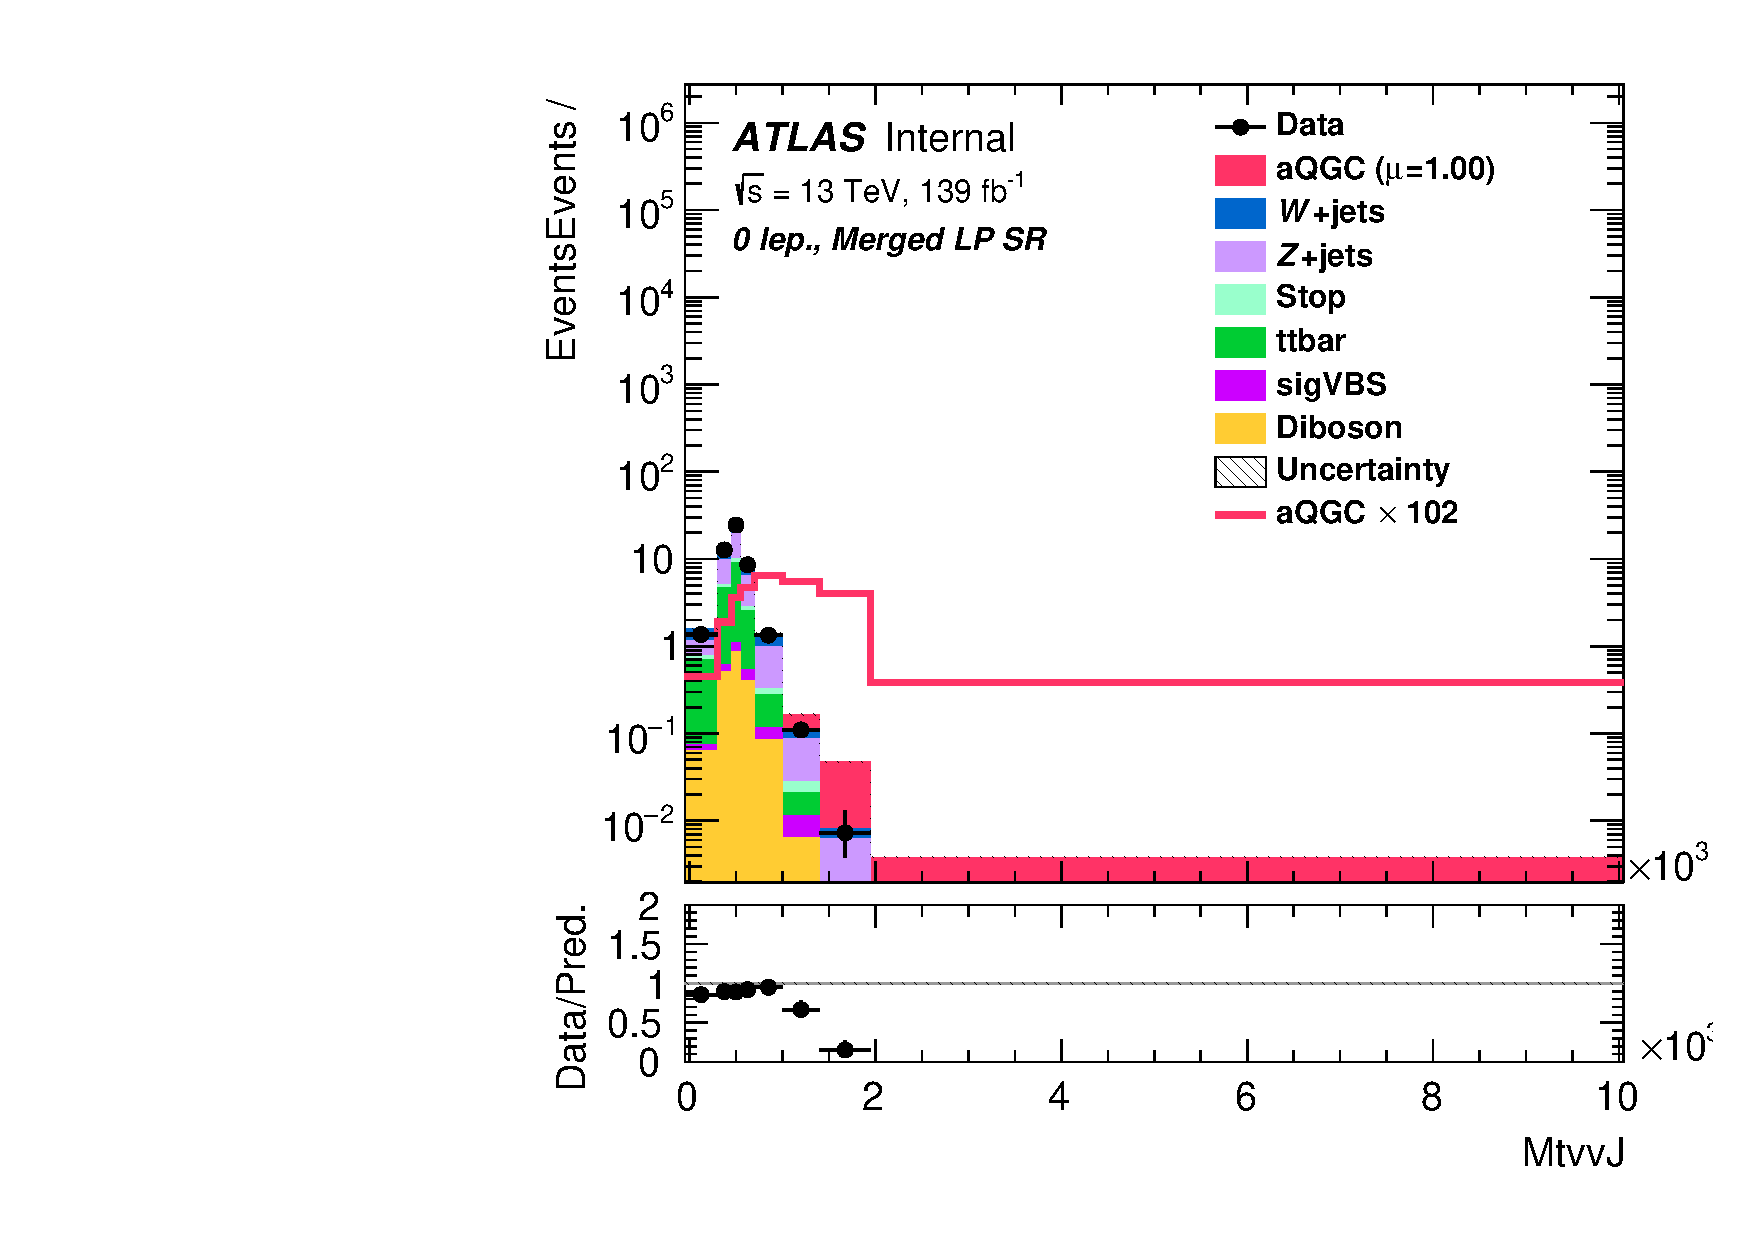
\includegraphics[width=0.32\textwidth]{figures/aQGC/Region_distMtvvJ_DSRVBSLP_BMin0_J0_incJet1_L0_T0_incFat1_Y6051_incTag1_Fat1_Prefitlog.pdf}}
%    	\subfigure[ 0lep resolved CR ]{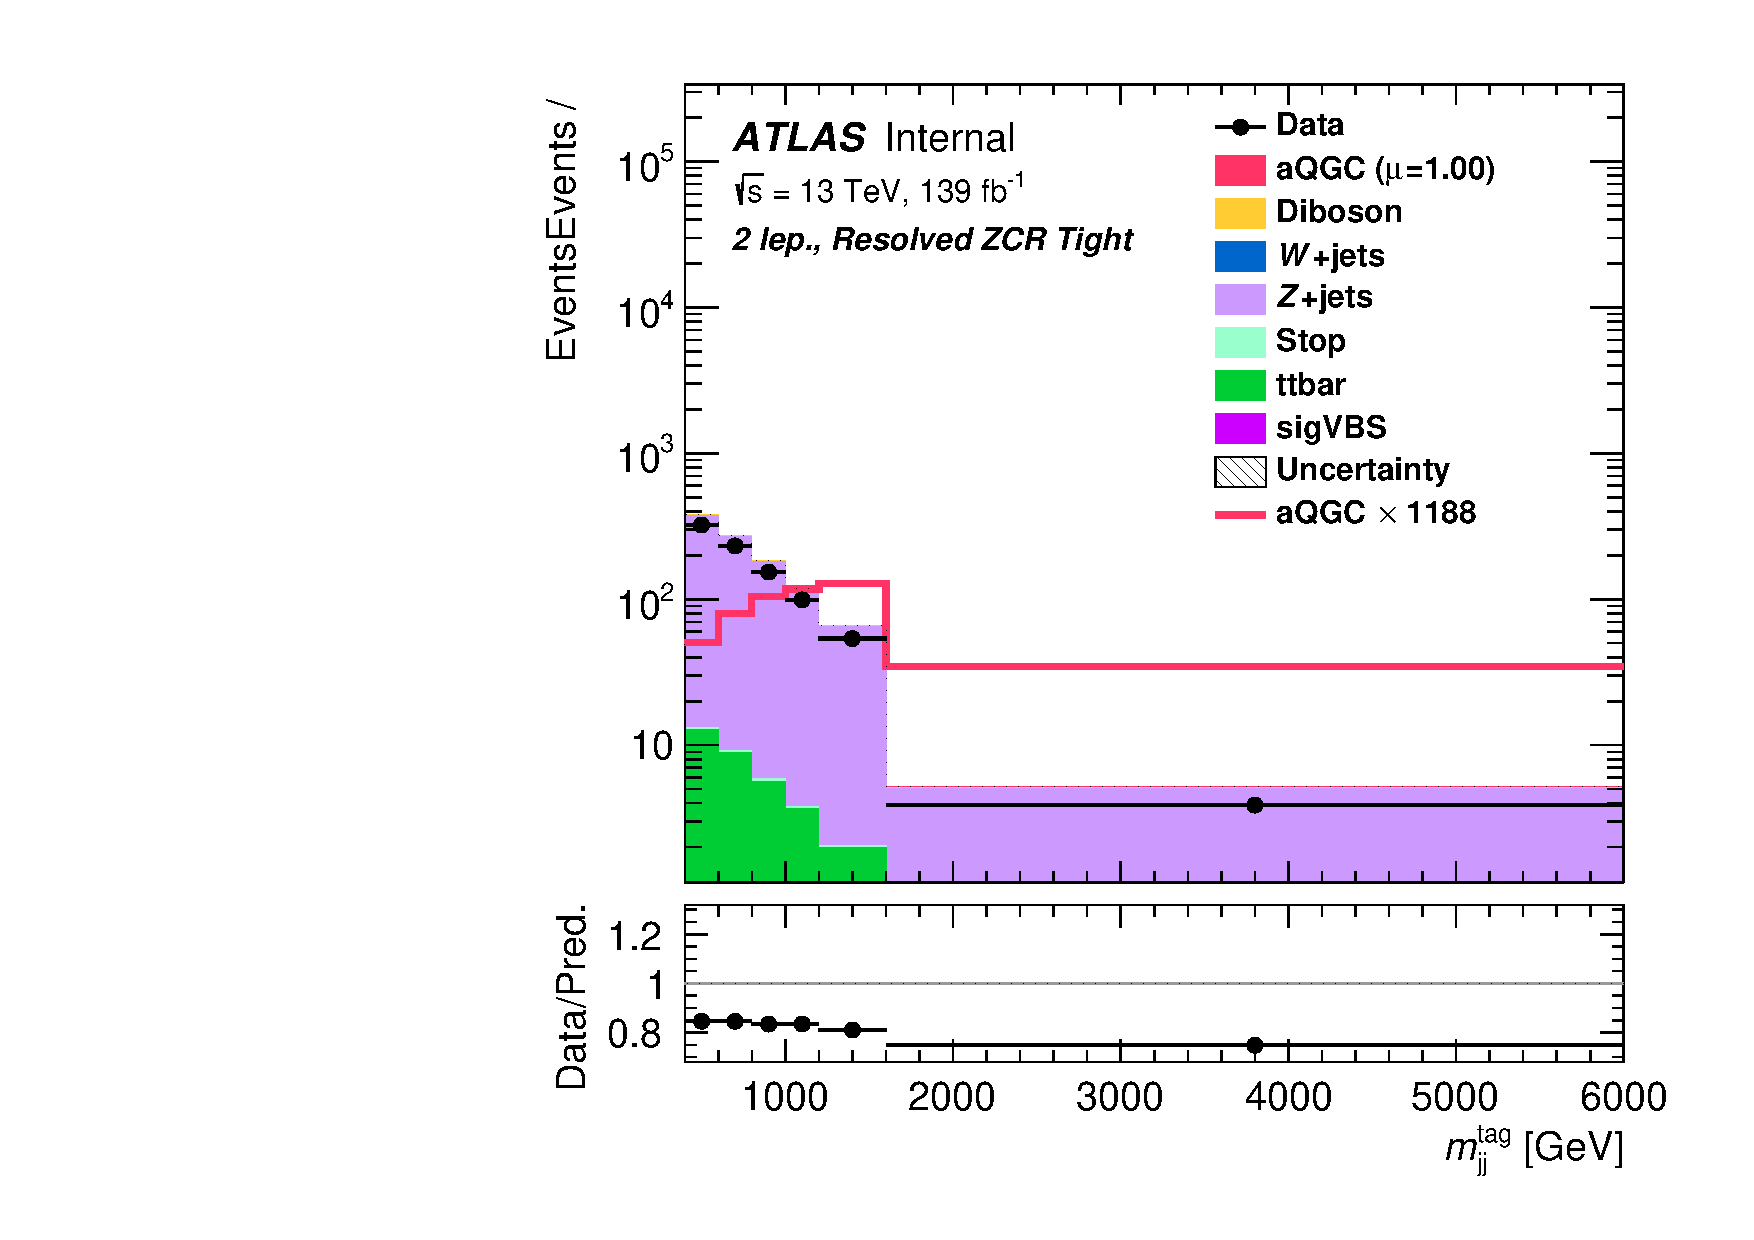
\includegraphics[width=0.32\textwidth]{figures/aQGC/Region_distMTagResJets_DCRVjetFid_BMin0_T0_Y6051_incTag1_J2_L2_incJet1_Prefitlog.pdf}}
%    	\subfigure[ 0lep resolved SR ]{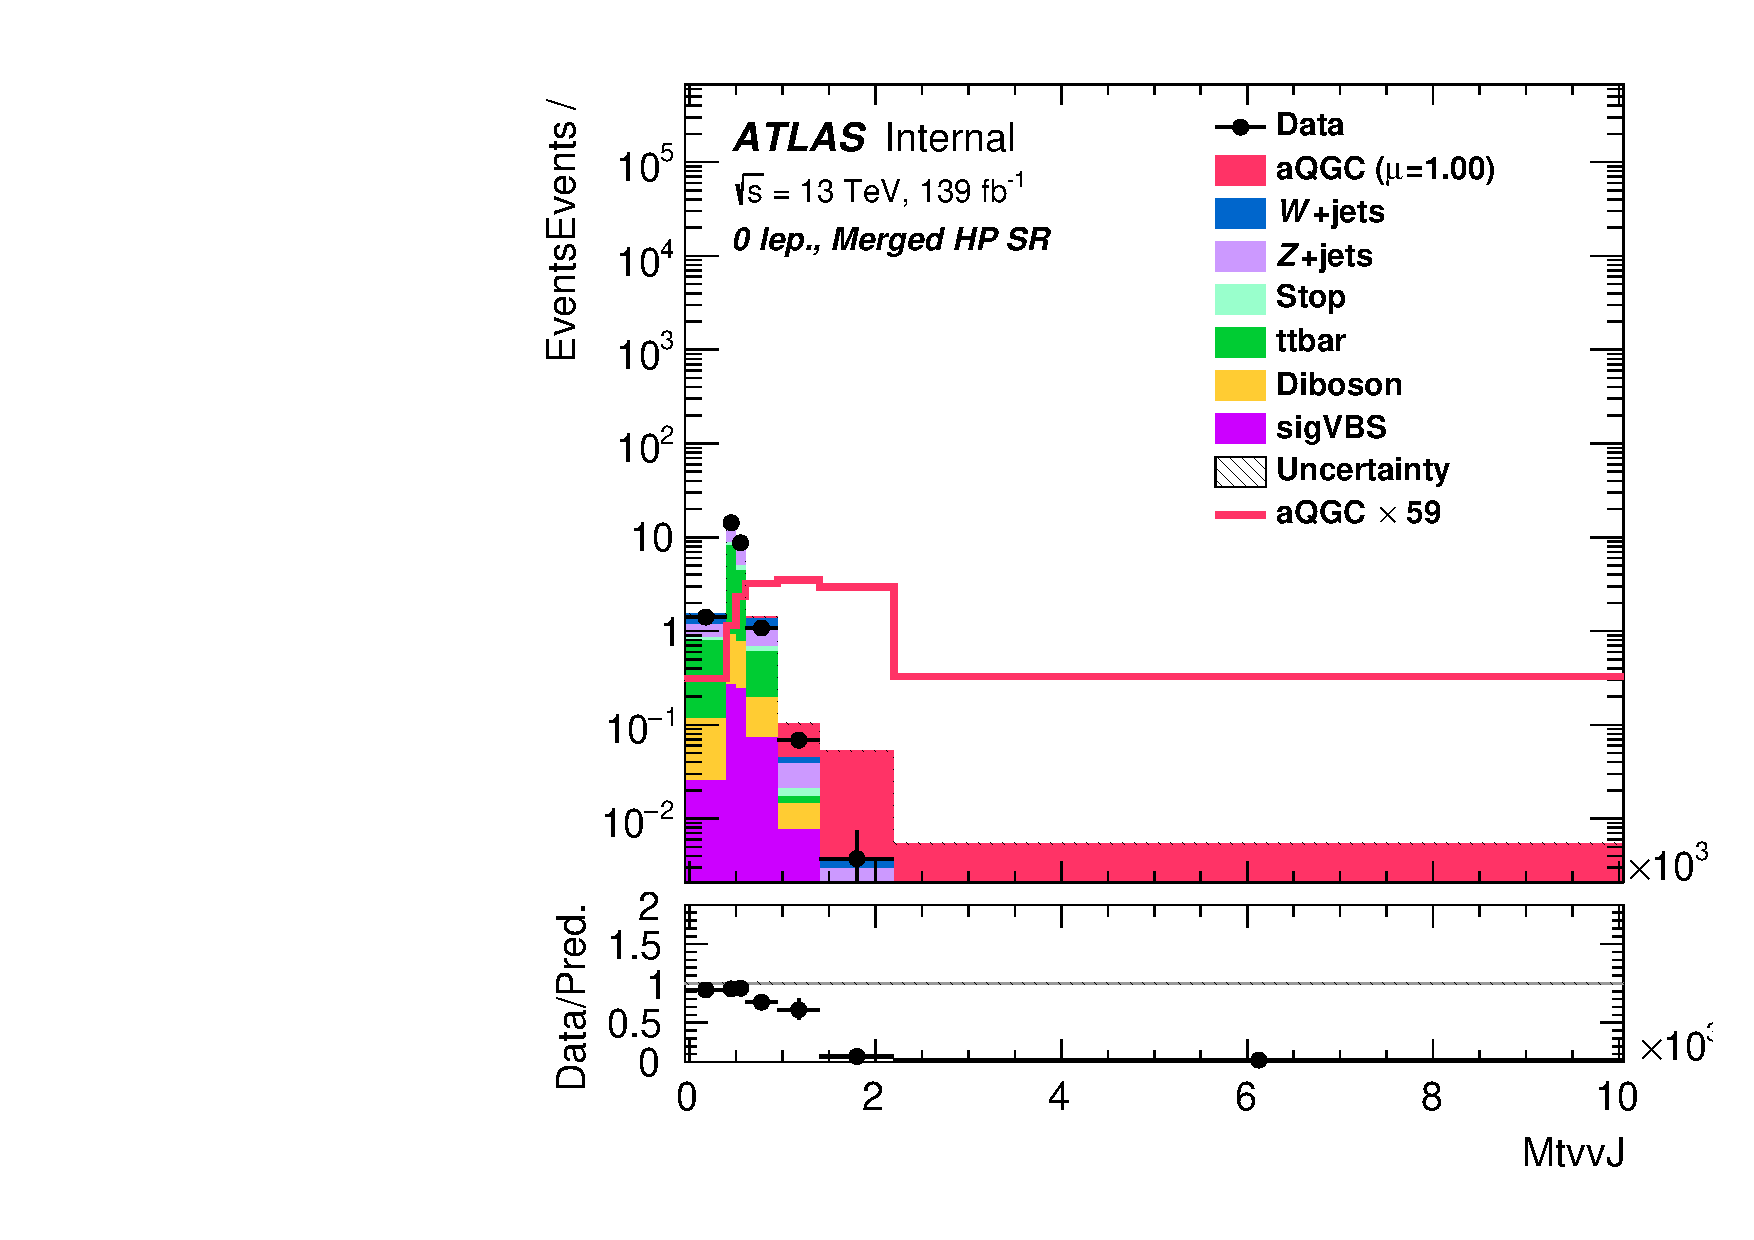
\includegraphics[width=0.32\textwidth]{figures/aQGC/Region_distMtvvJ_DSRVBSHP_BMin0_J0_incJet1_L0_T0_incFat1_Y6051_incTag1_Fat1_Prefitlog.pdf}}
%        \caption{Prefit plots for operator FT0 in \zlep channel are shown. The standard model EW signal is floated as the background.}
%        \label{fig:0lepFT0}
%\end{figure}
%
%\begin{figure}[ht]
%    \centering
%    	\subfigure[ 1lep merged Vjet CR ]{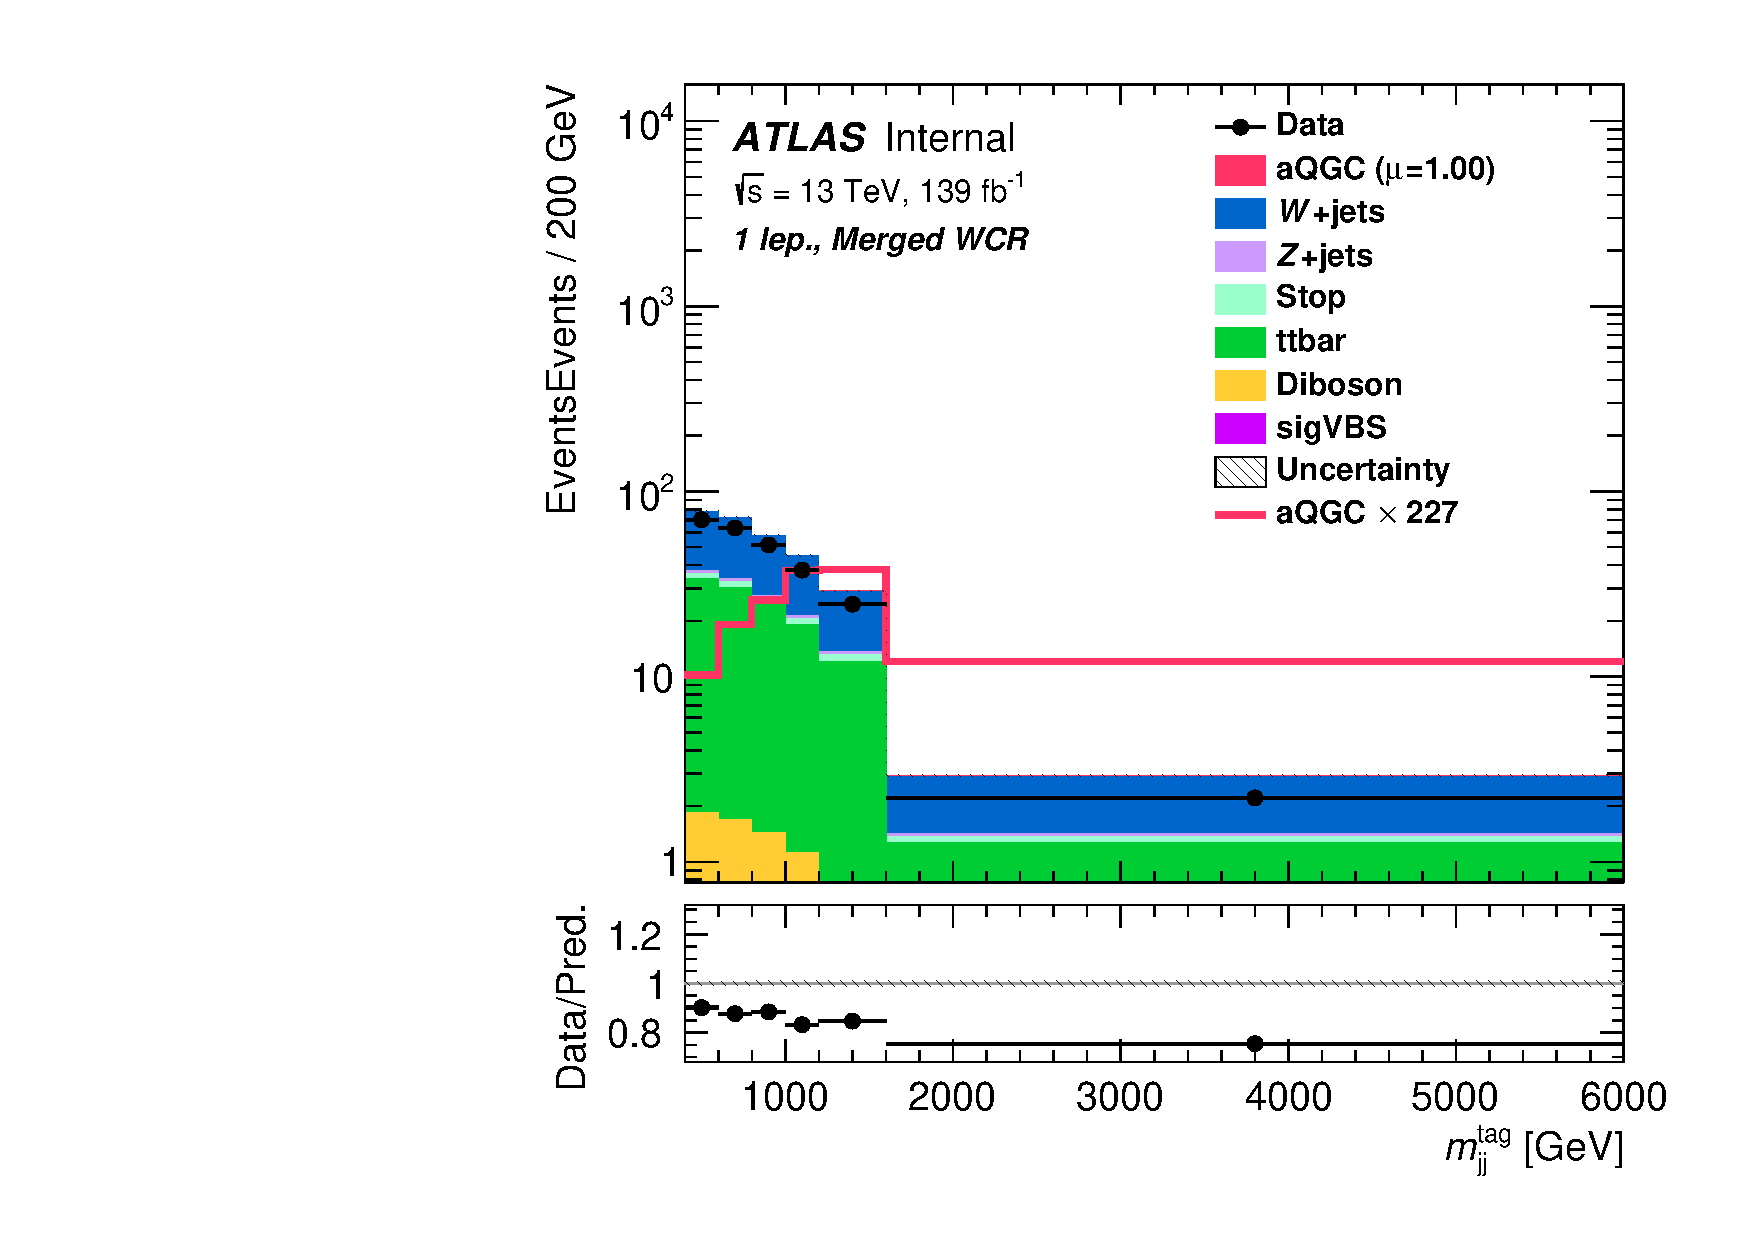
\includegraphics[width=0.32\textwidth]{figures/aQGC/Region_disttagMjj_DCRVjetMerged_BMin0_J0_incJet1_L1_T0_incFat1_Y6051_incTag1_Fat1_Prefitlog.pdf}}
%    	\subfigure[ 1lep HP Top CR ]{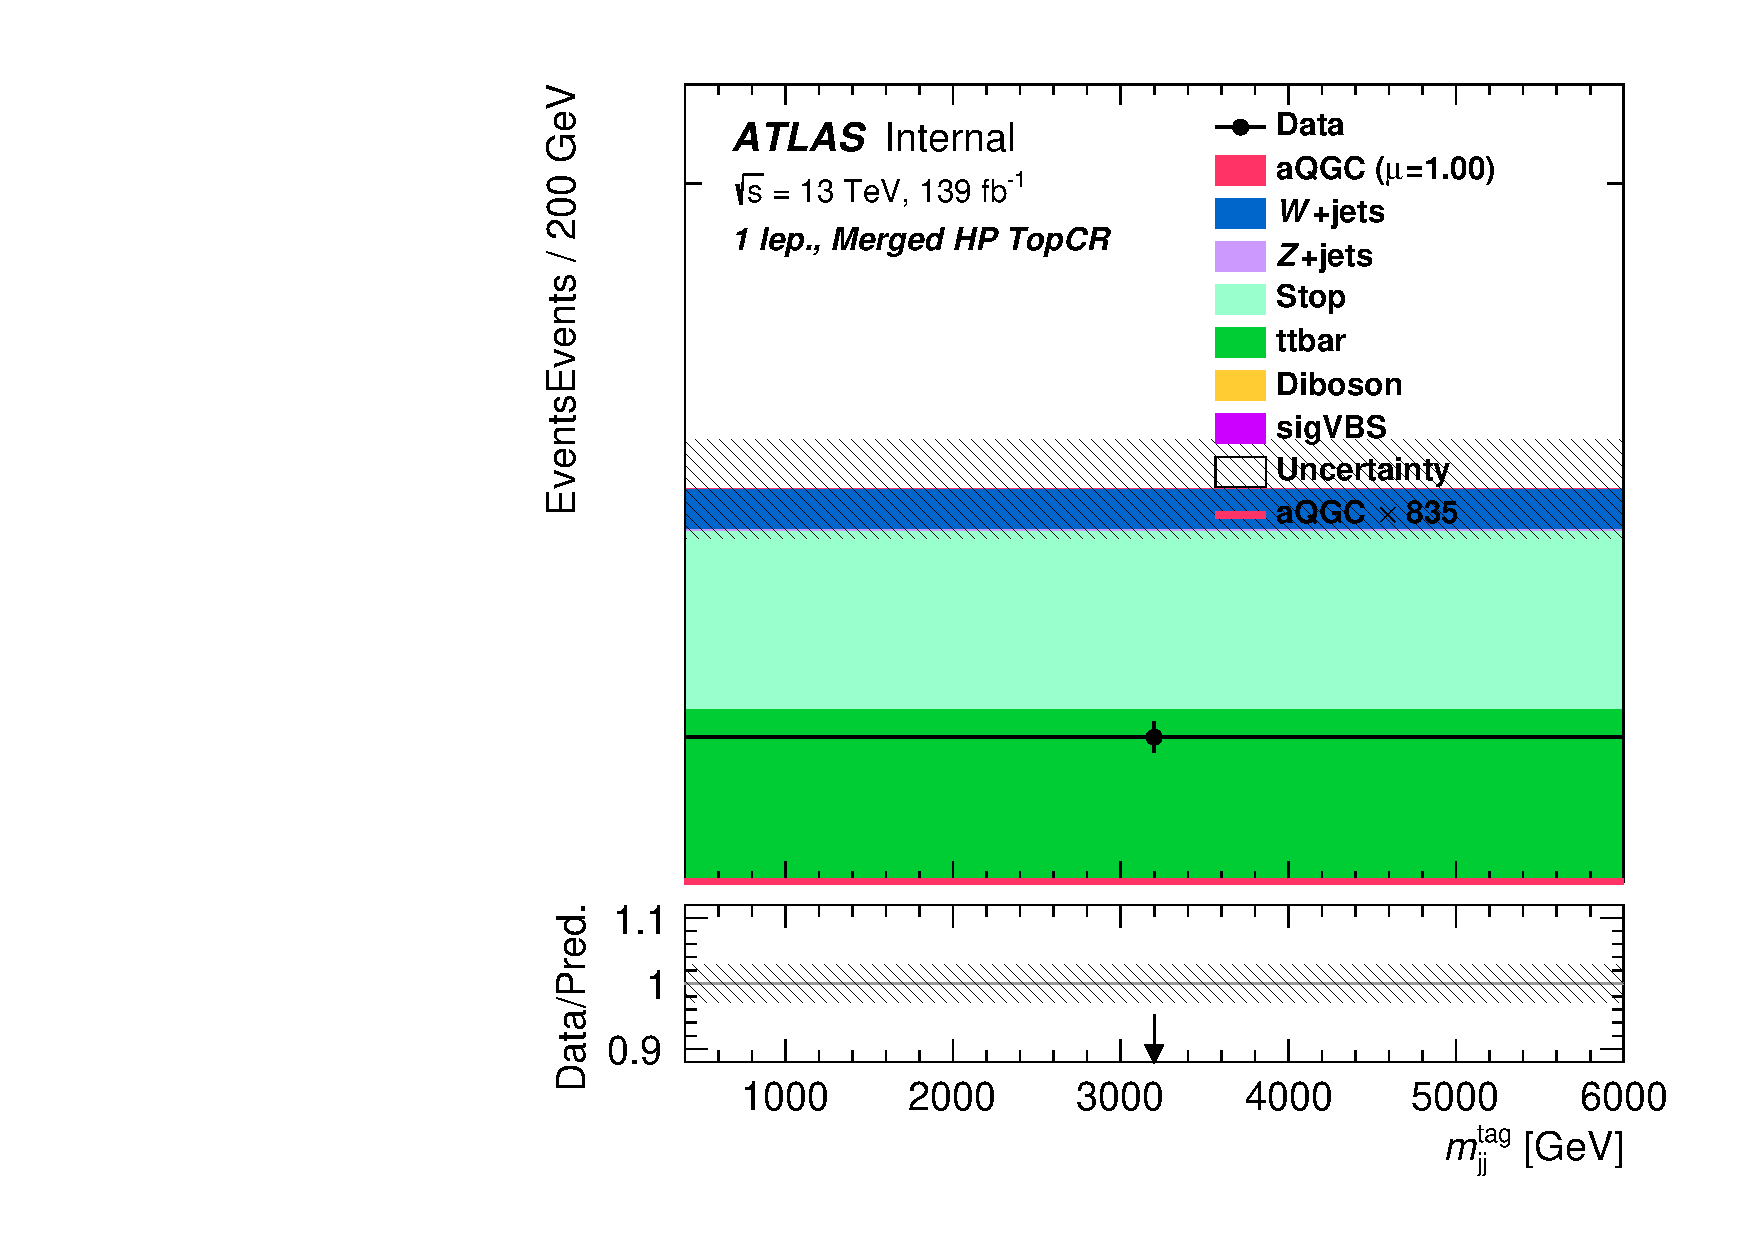
\includegraphics[width=0.32\textwidth]{figures/aQGC/Region_disttagMjj_DCRTopHP_BMin0_J0_incJet1_L1_T0_incFat1_Y6051_incTag1_Fat1_Prefitlog.pdf}}
%    	\subfigure[ 1lep LP Top CR ]{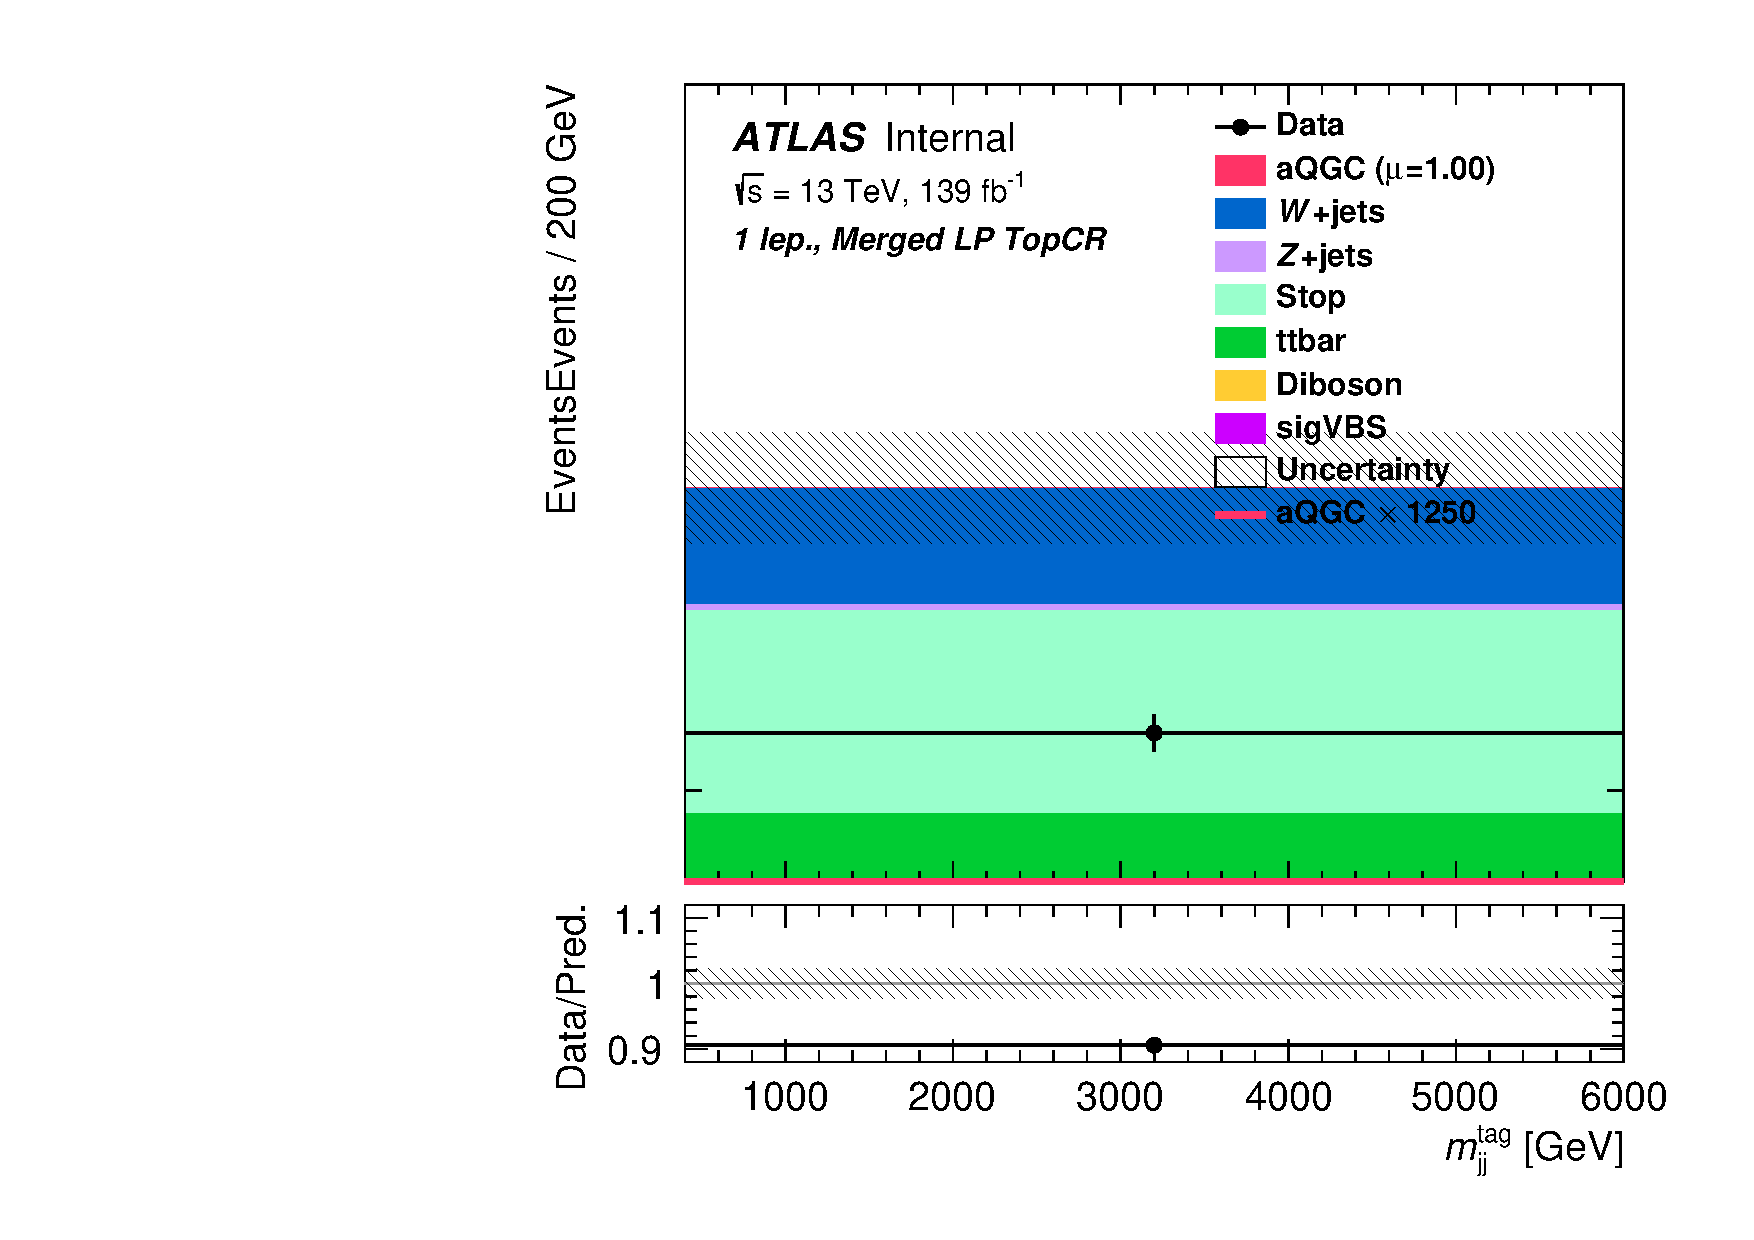
\includegraphics[width=0.32\textwidth]{figures/aQGC/Region_disttagMjj_DCRTopLP_BMin0_J0_incJet1_L1_T0_incFat1_Y6051_incTag1_Fat1_Prefitlog.pdf}}
%    	\subfigure[ 1lep HP SR ]{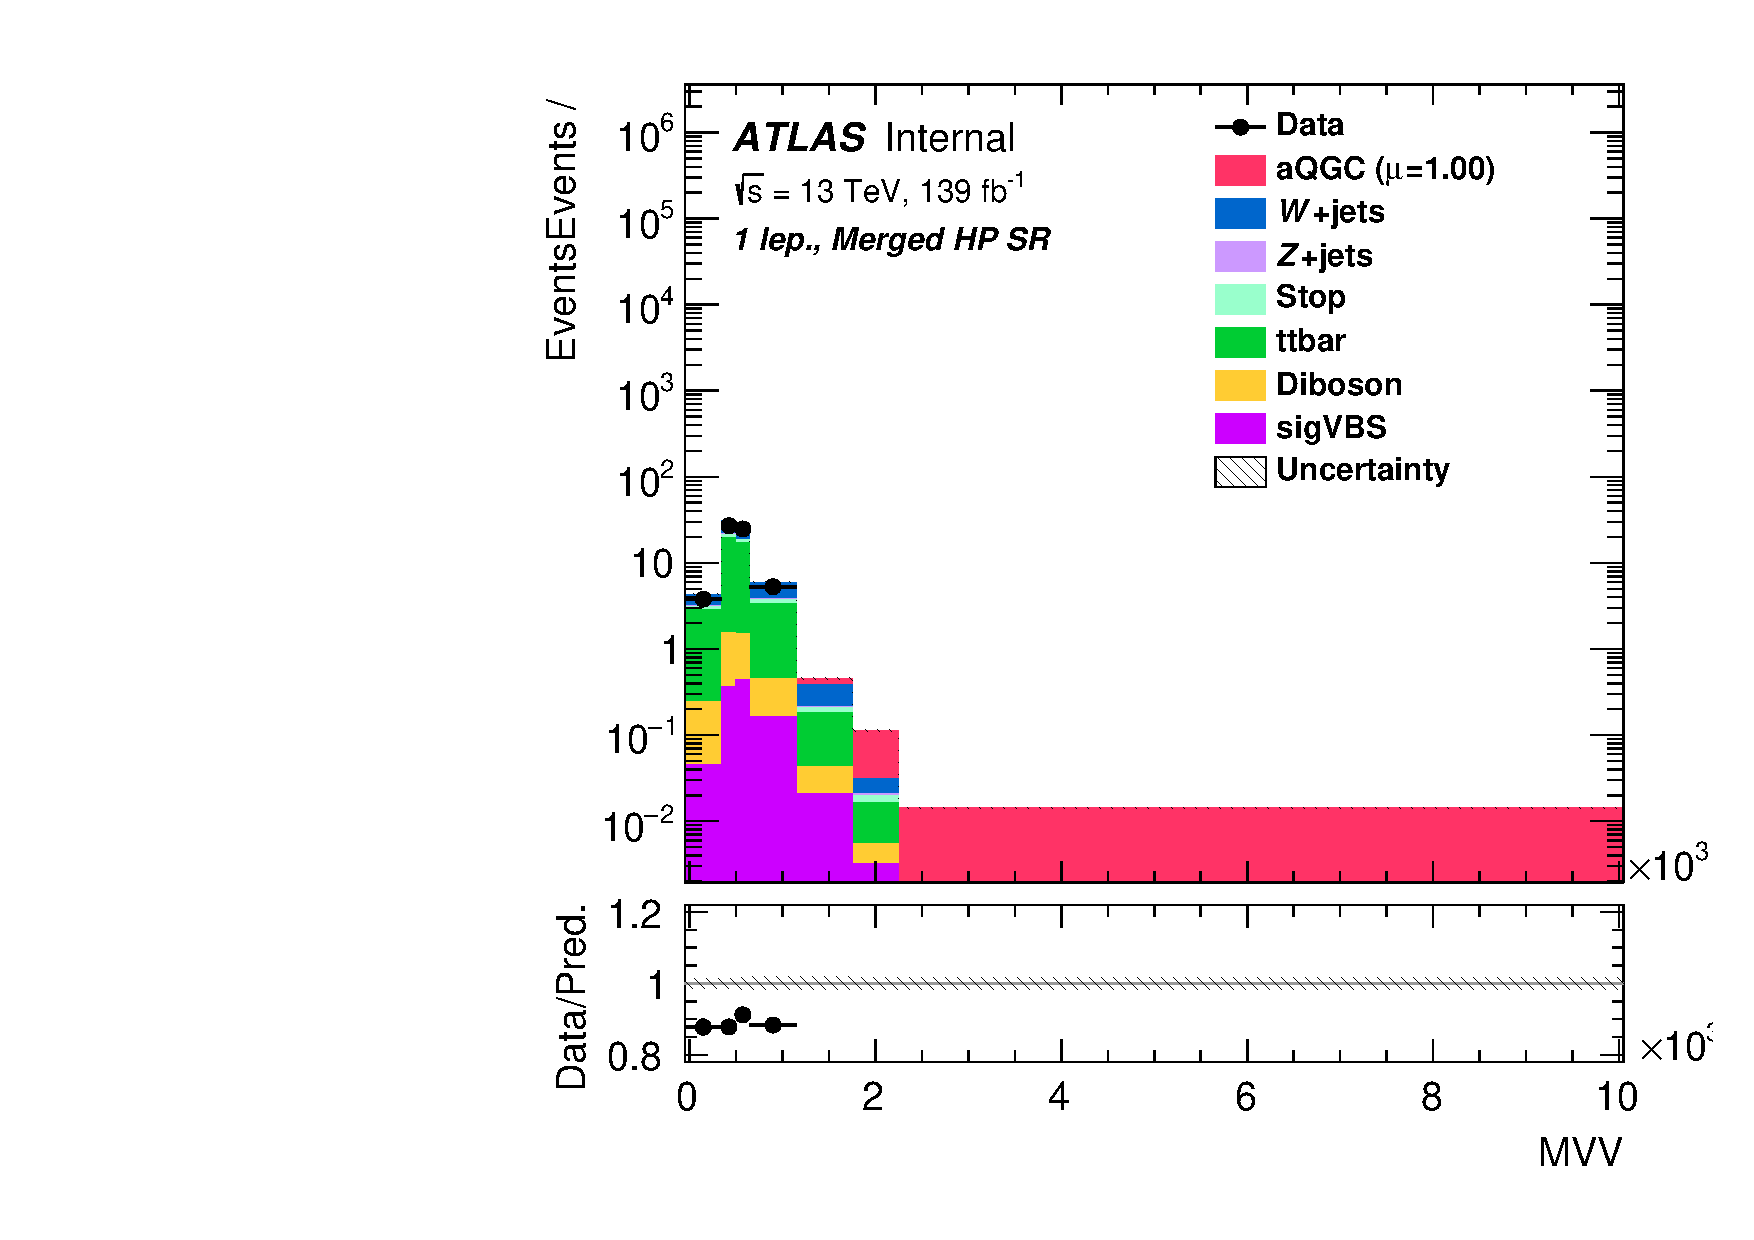
\includegraphics[width=0.32\textwidth]{figures/aQGC/Region_distMVV_DSRVBSHP_BMin0_J0_incJet1_L1_T0_incFat1_Y6051_incTag1_Fat1_Prefitlog.pdf}}
%    	\subfigure[ 1lep LP SR ]{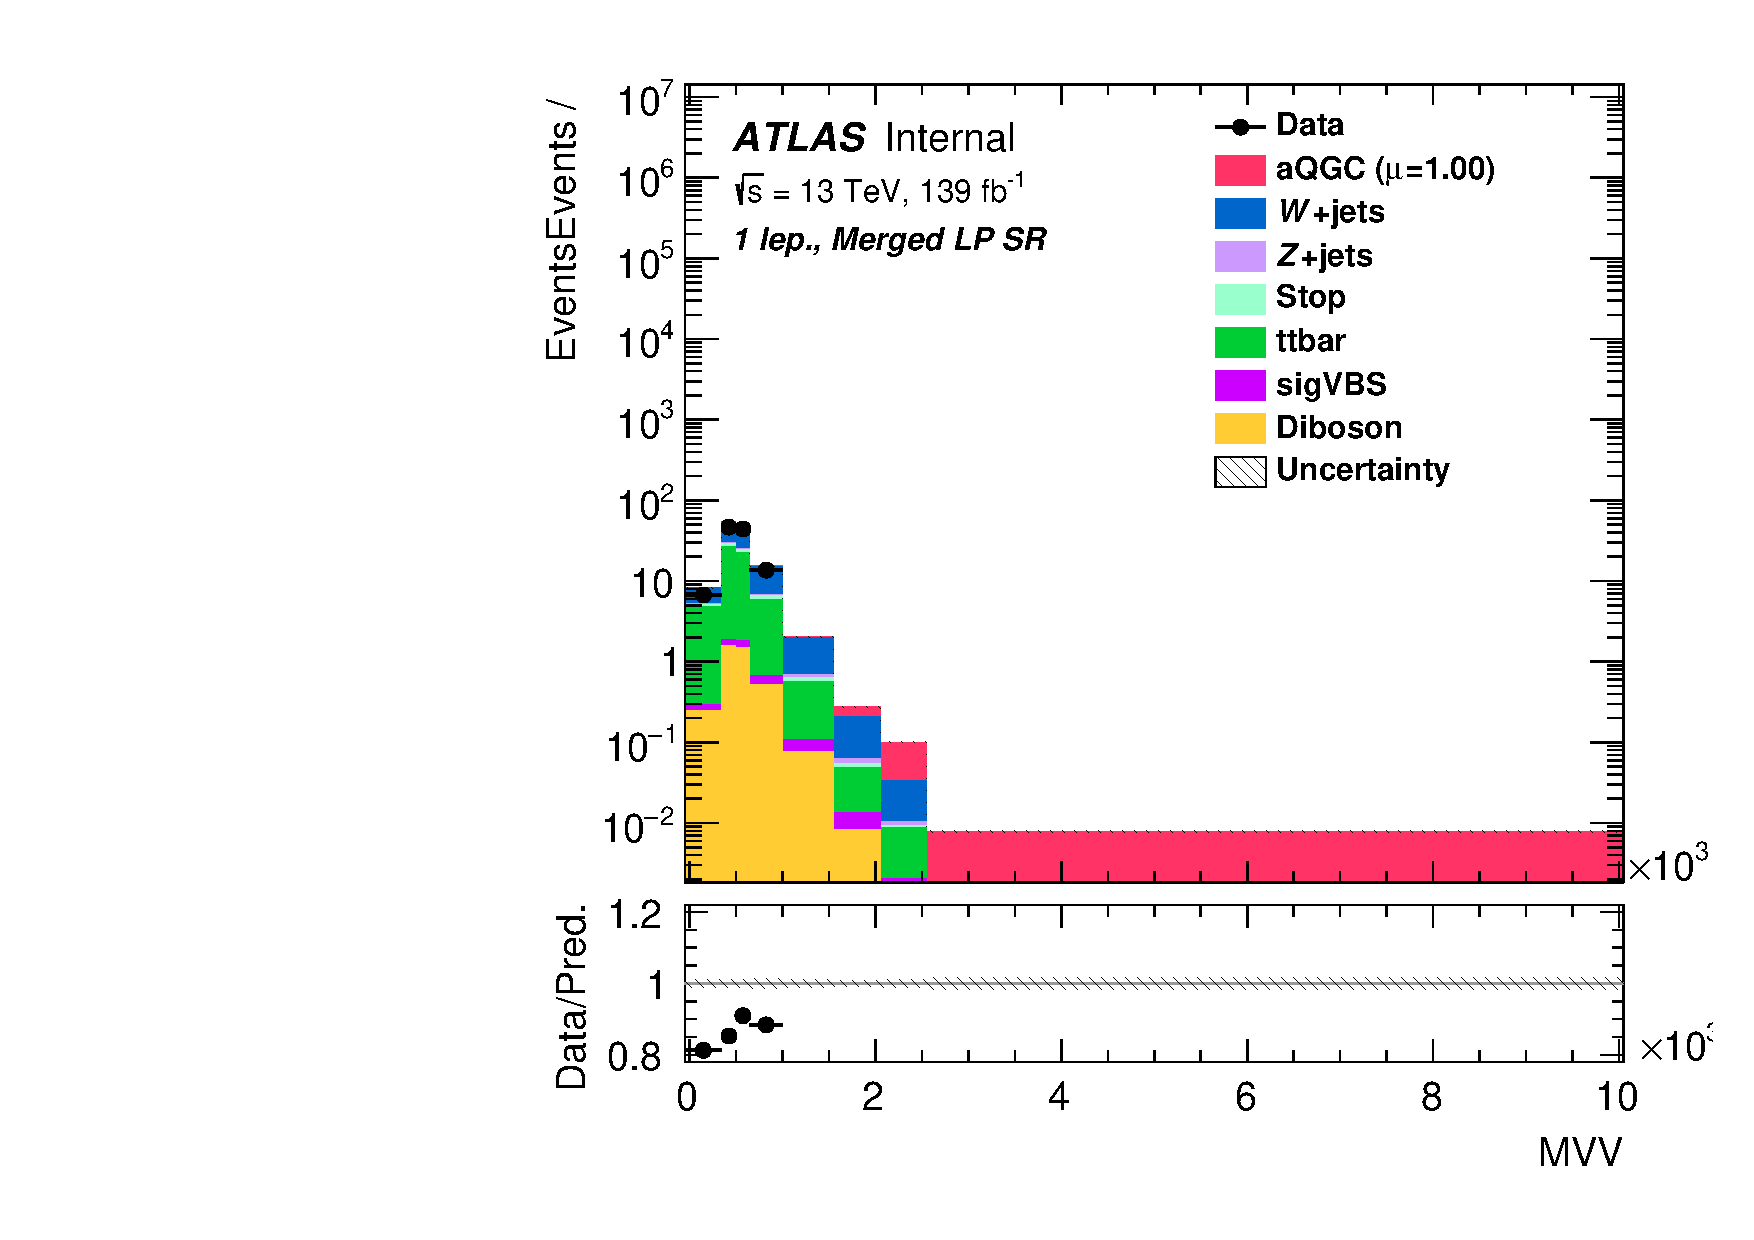
\includegraphics[width=0.32\textwidth]{figures/aQGC/Region_distMVV_DSRVBSLP_BMin0_J0_incJet1_L1_T0_incFat1_Y6051_incTag1_Fat1_Prefitlog.pdf}}
%    	\subfigure[ 1lep resolved Vjet CR ]{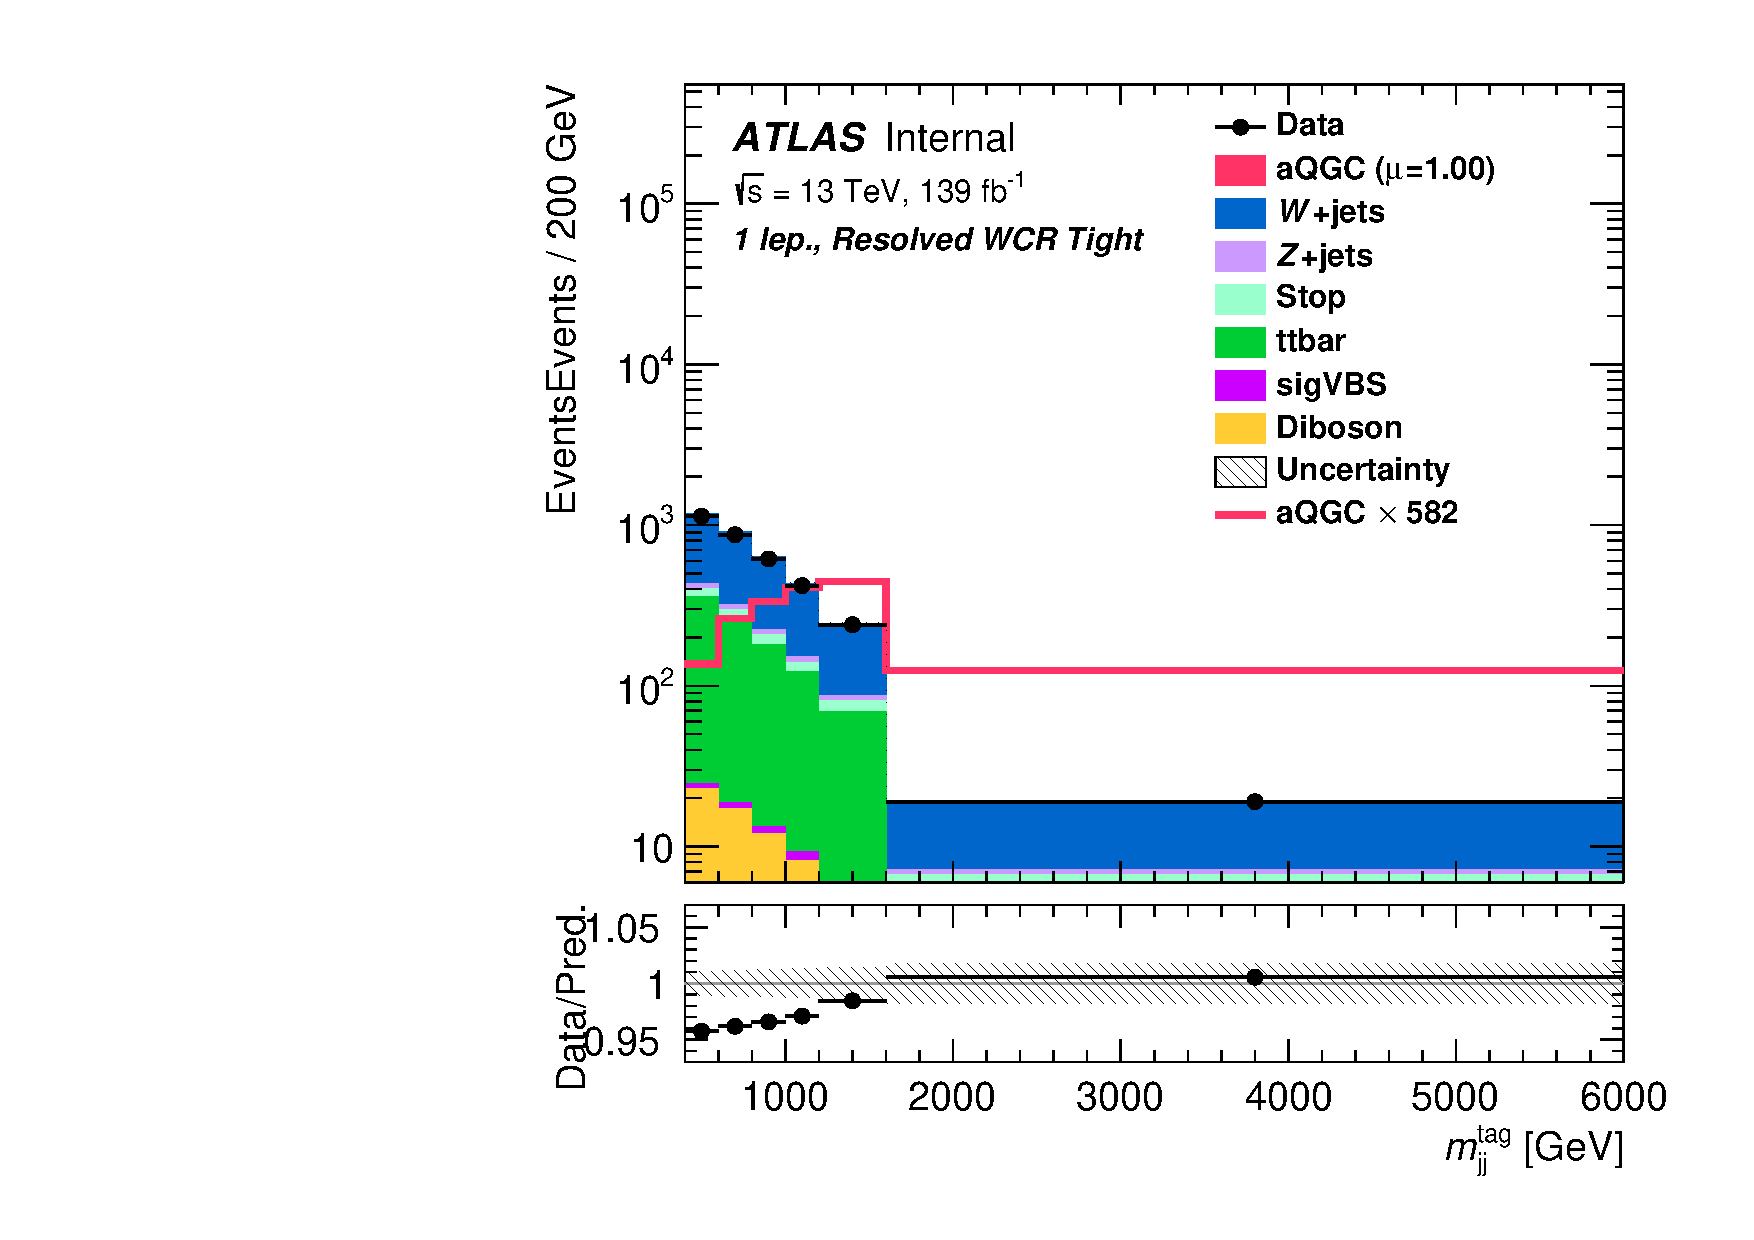
\includegraphics[width=0.32\textwidth]{figures/aQGC/Region_disttagMjj_DCRVjetTight_BMin0_T0_Y6051_incTag1_J2_L1_incJet1_Prefitlog.pdf}}
%    	\subfigure[ 1lep resolved Top CR ]{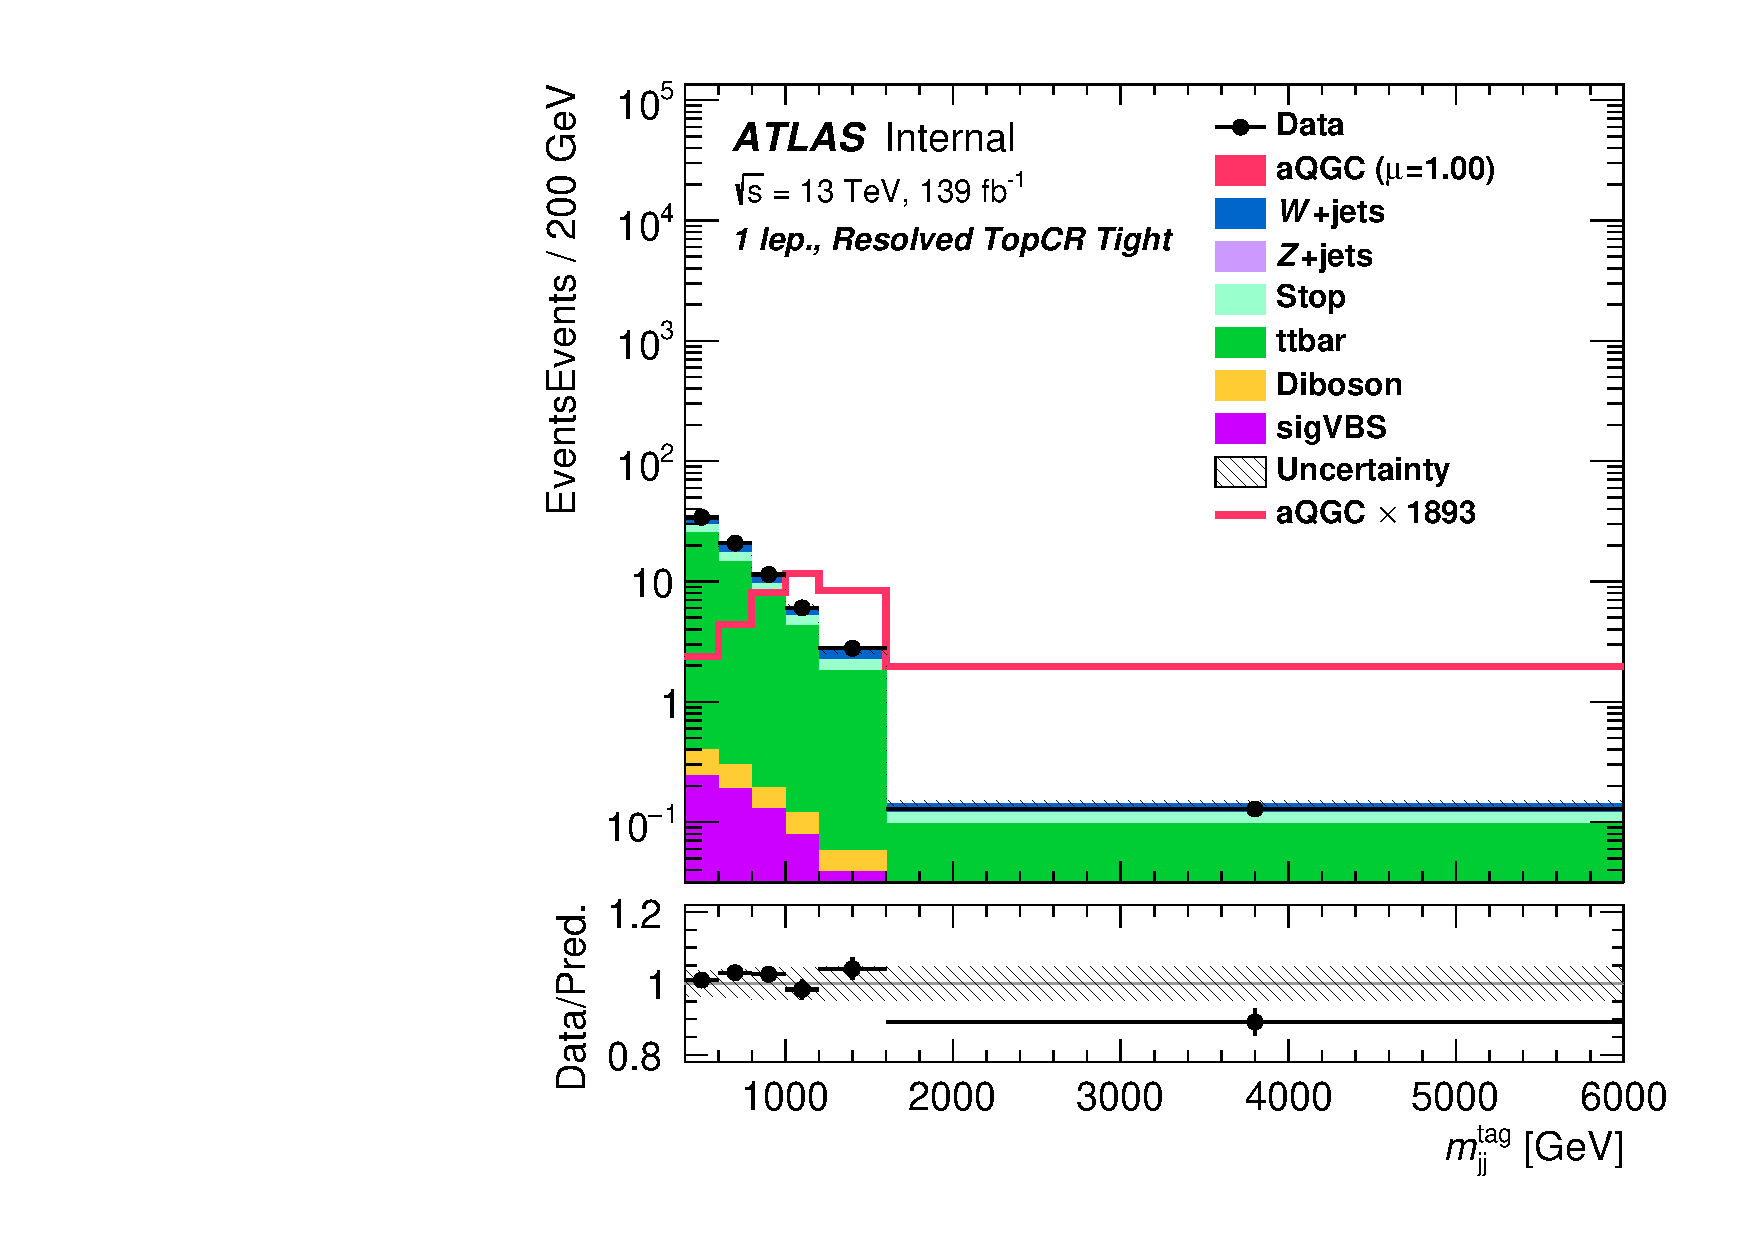
\includegraphics[width=0.32\textwidth]{figures/aQGC/Region_disttagMjj_DCRTopTight_BMin0_T0_Y6051_incTag1_J2_L1_incJet1_Prefitlog.pdf}}
%    	\subfigure[ 1lep resolved SR ]{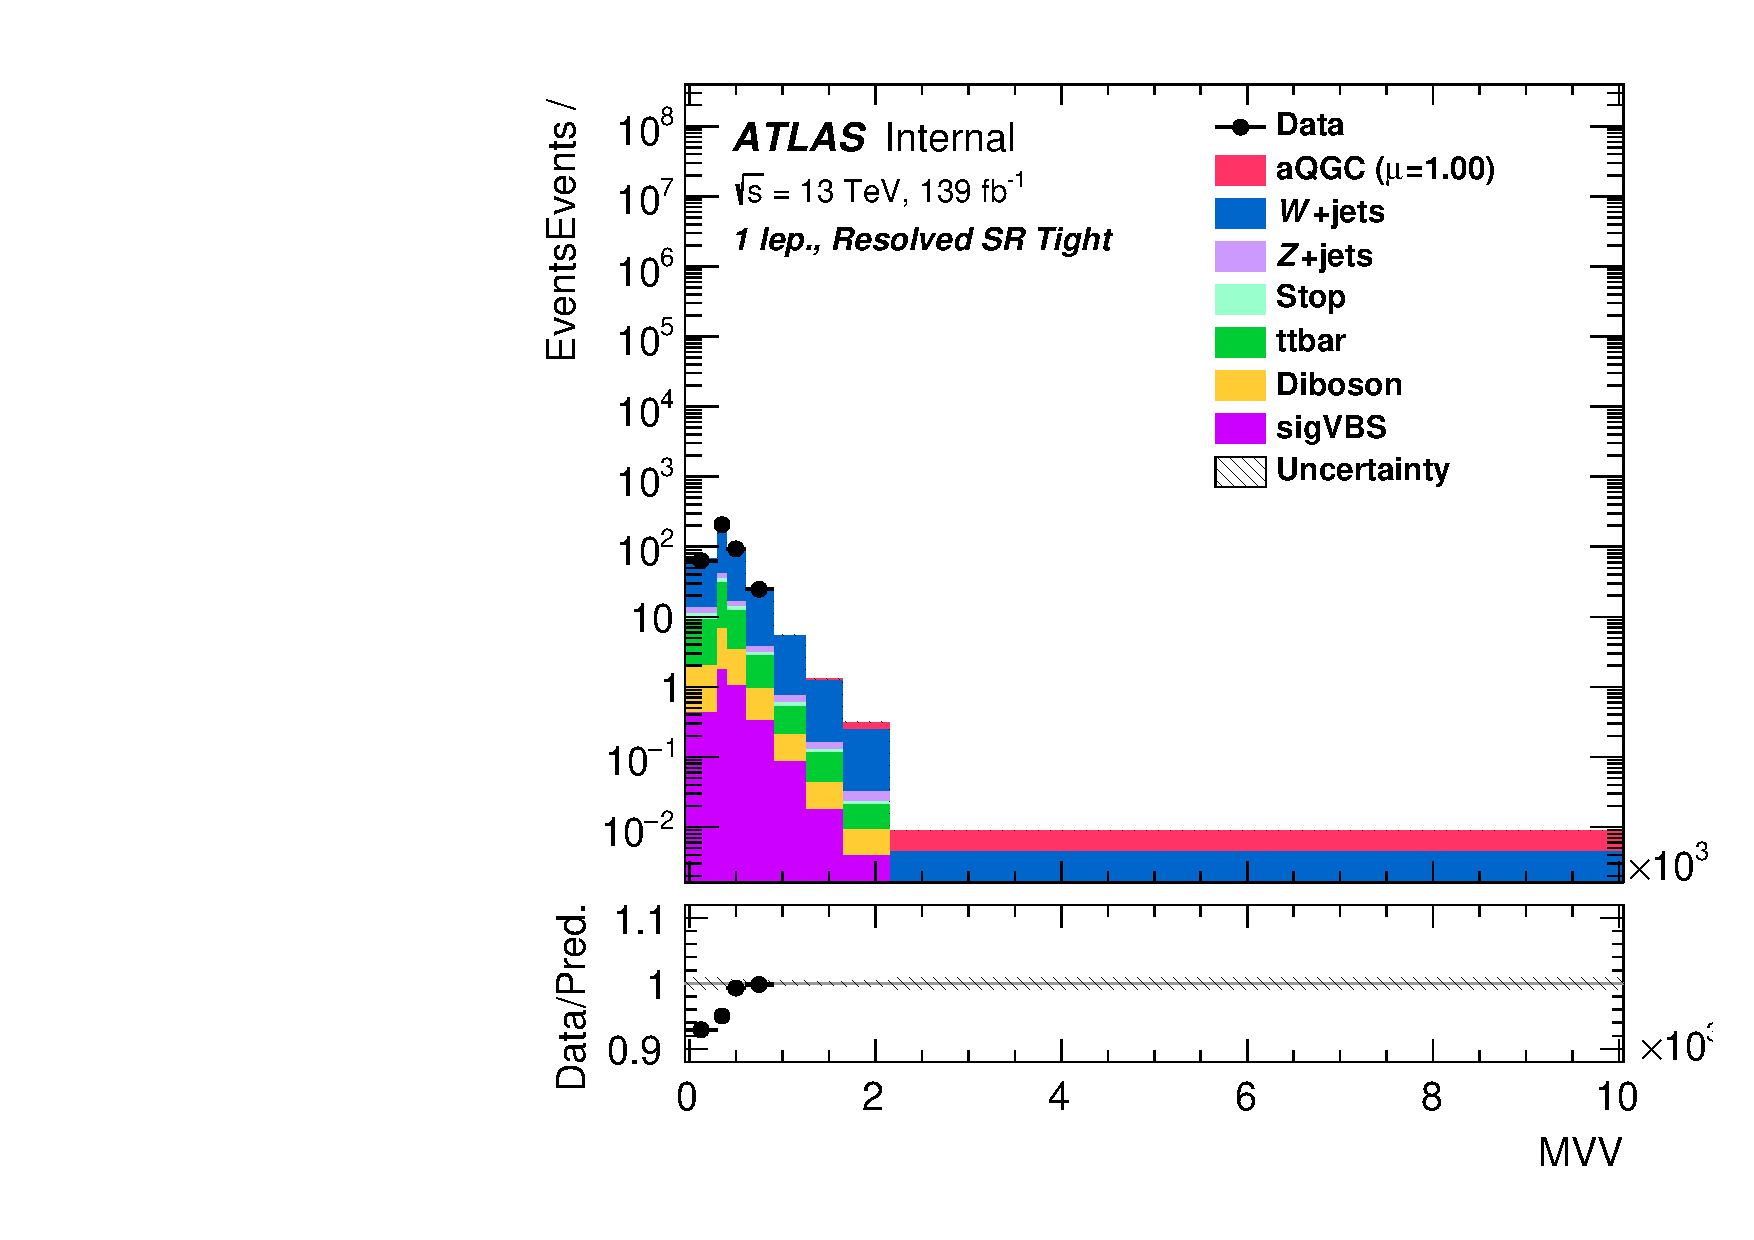
\includegraphics[width=0.32\textwidth]{figures/aQGC/Region_distMVV_DSRVBSTight_BMin0_T0_Y6051_incTag1_J2_L1_incJet1_Prefitlog.pdf}}
%        \caption{Prefit plots for operator FT0 in \olep channel are shown. The standard model EW signal is floated as the background.}
%        \label{fig:1lepFT0}
%\end{figure}
%
%\begin{figure}[ht]
%    \centering
%    	\subfigure[ 2lep merged CR ]{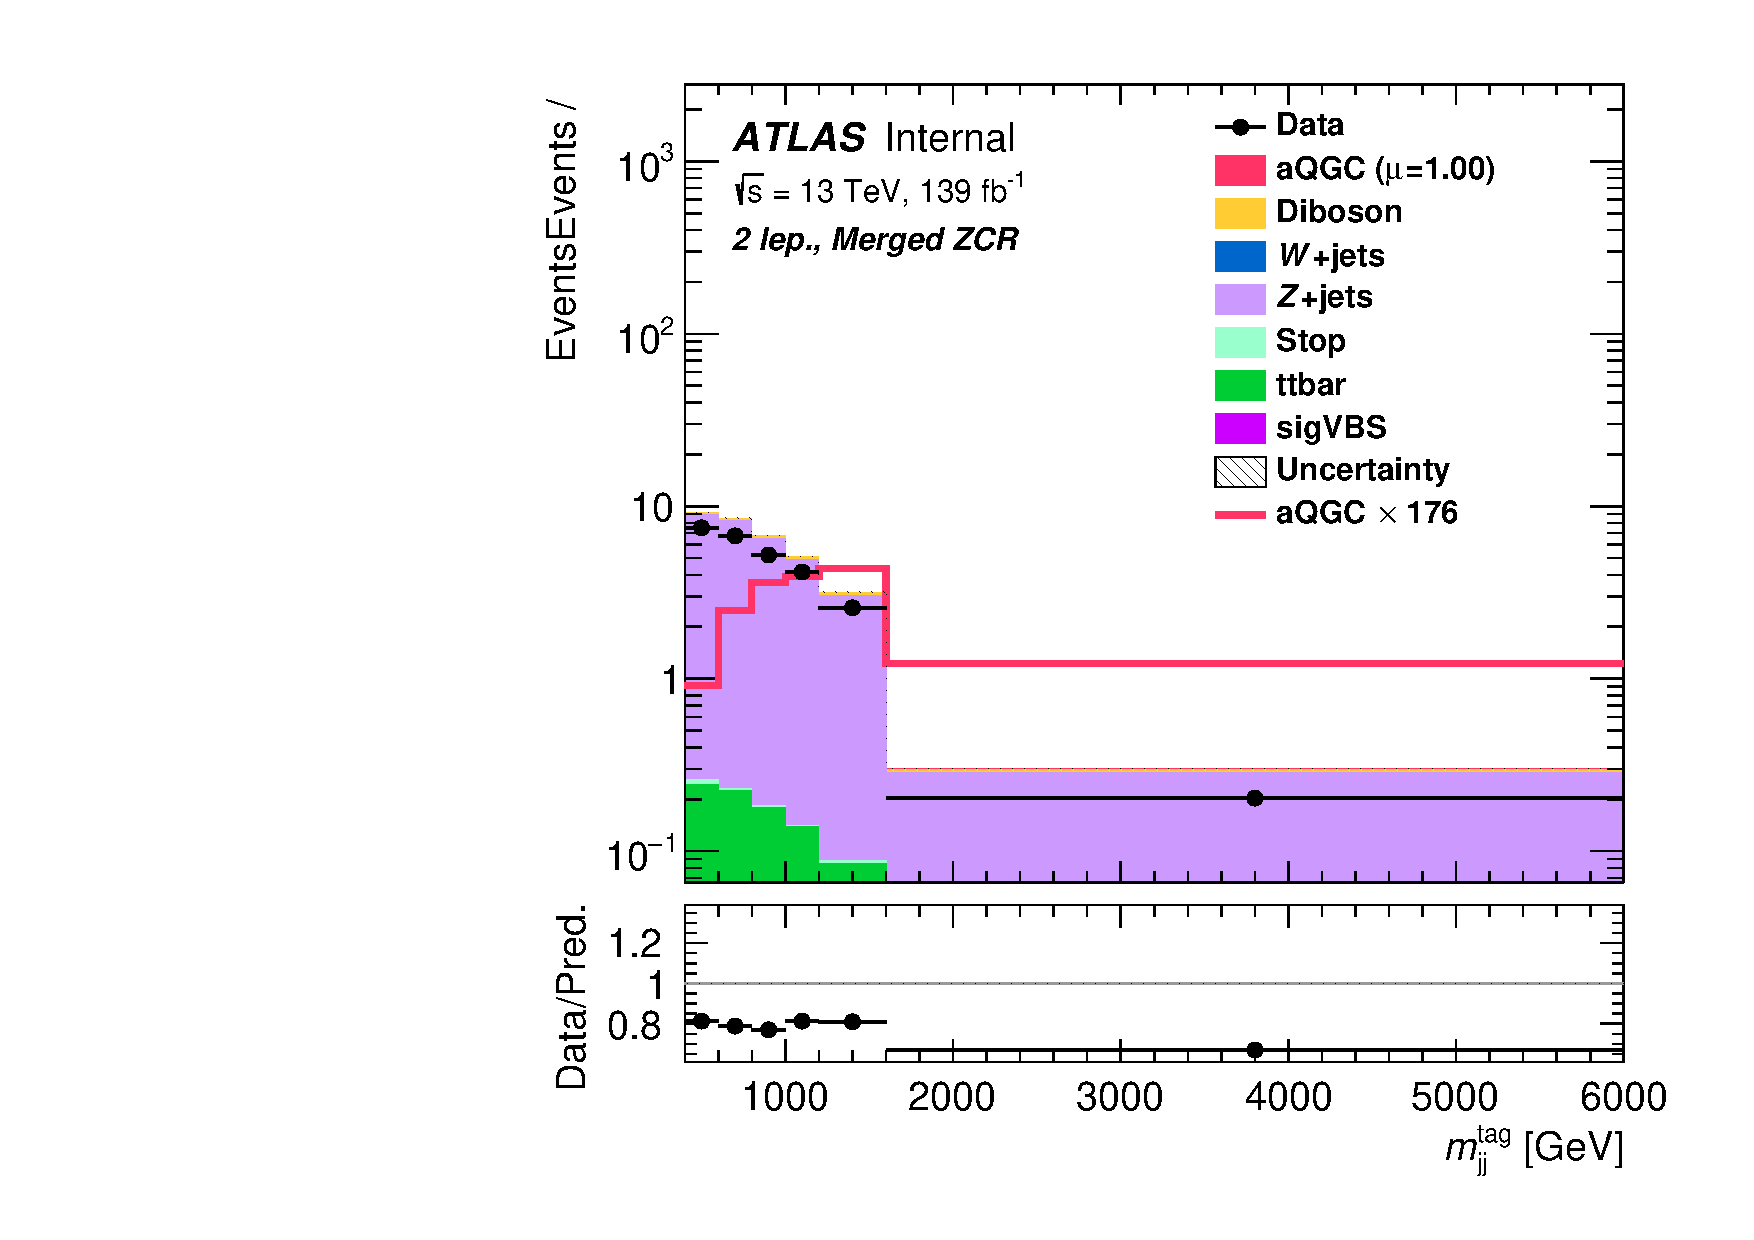
\includegraphics[width=0.32\textwidth]{figures/aQGC/Region_distMTagMerJets_DCRVjet_BMin0_J0_incJet1_L2_T0_incFat1_Y6051_incTag1_Fat1_Prefitlog.pdf}}
%    	\subfigure[ 2lep HP SR ]{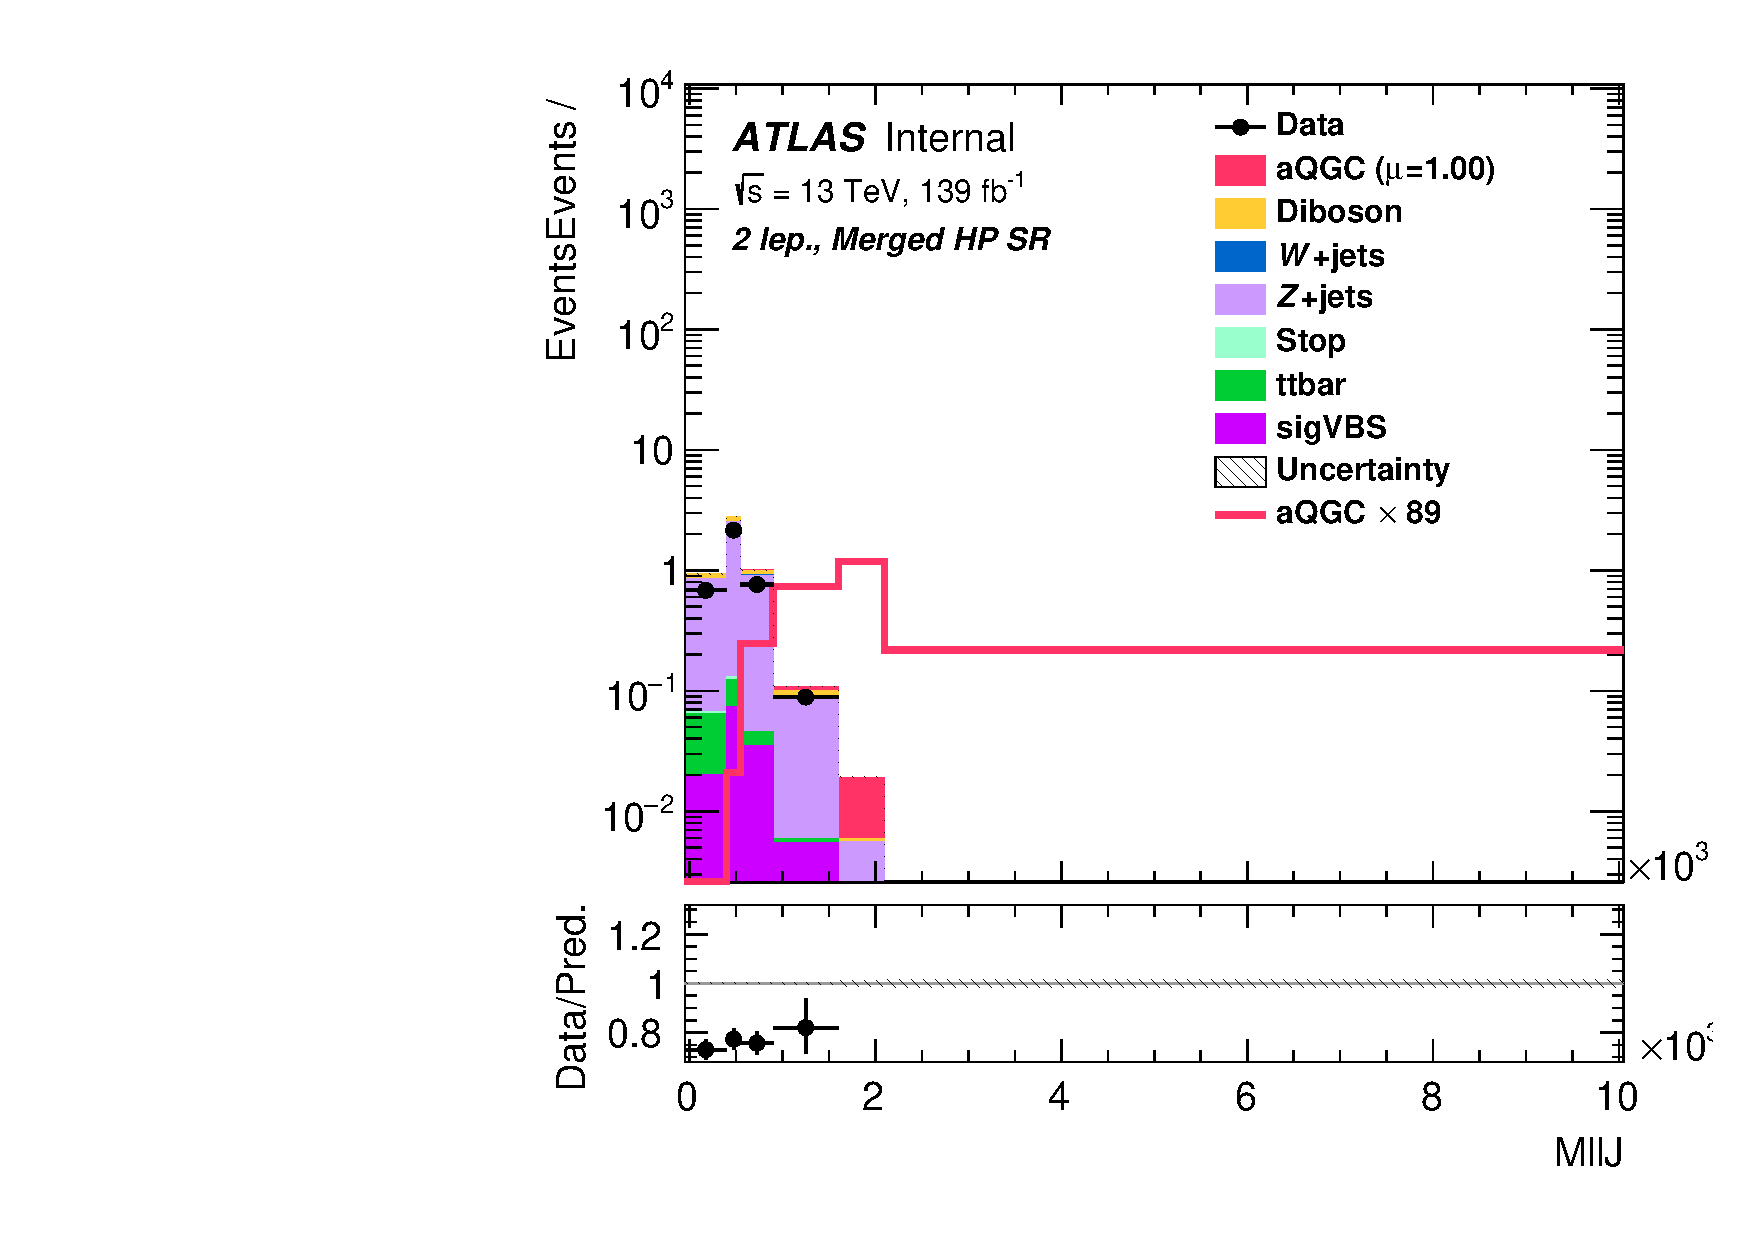
\includegraphics[width=0.32\textwidth]{figures/aQGC/Region_distMllJ_DSRVBSHP_BMin0_J0_incJet1_L2_T0_incFat1_Y6051_incTag1_Fat1_Prefitlog.pdf}}
%    	\subfigure[ 2lep LP SR ]{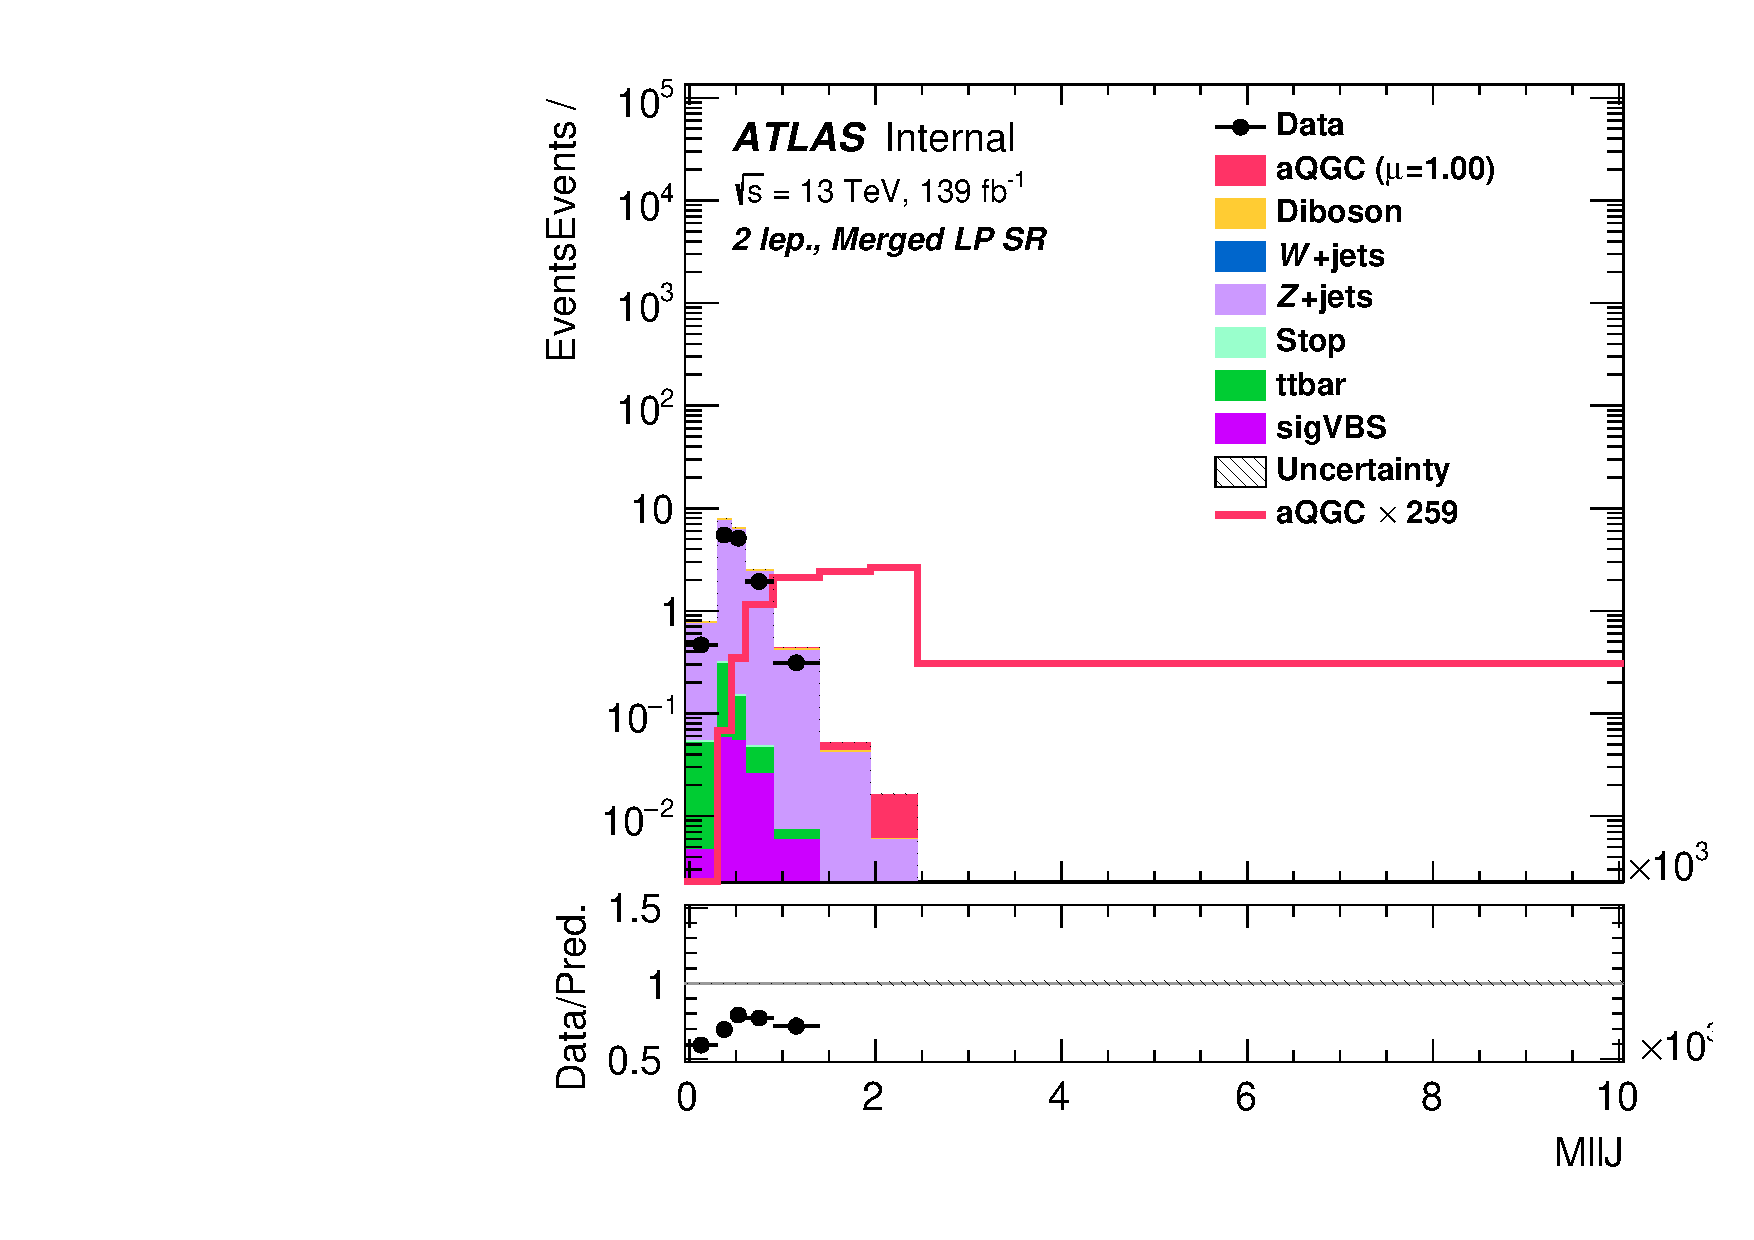
\includegraphics[width=0.32\textwidth]{figures/aQGC/Region_distMllJ_DSRVBSLP_BMin0_J0_incJet1_L2_T0_incFat1_Y6051_incTag1_Fat1_Prefitlog.pdf}}
%    	\subfigure[ 2lep resolved CR ]{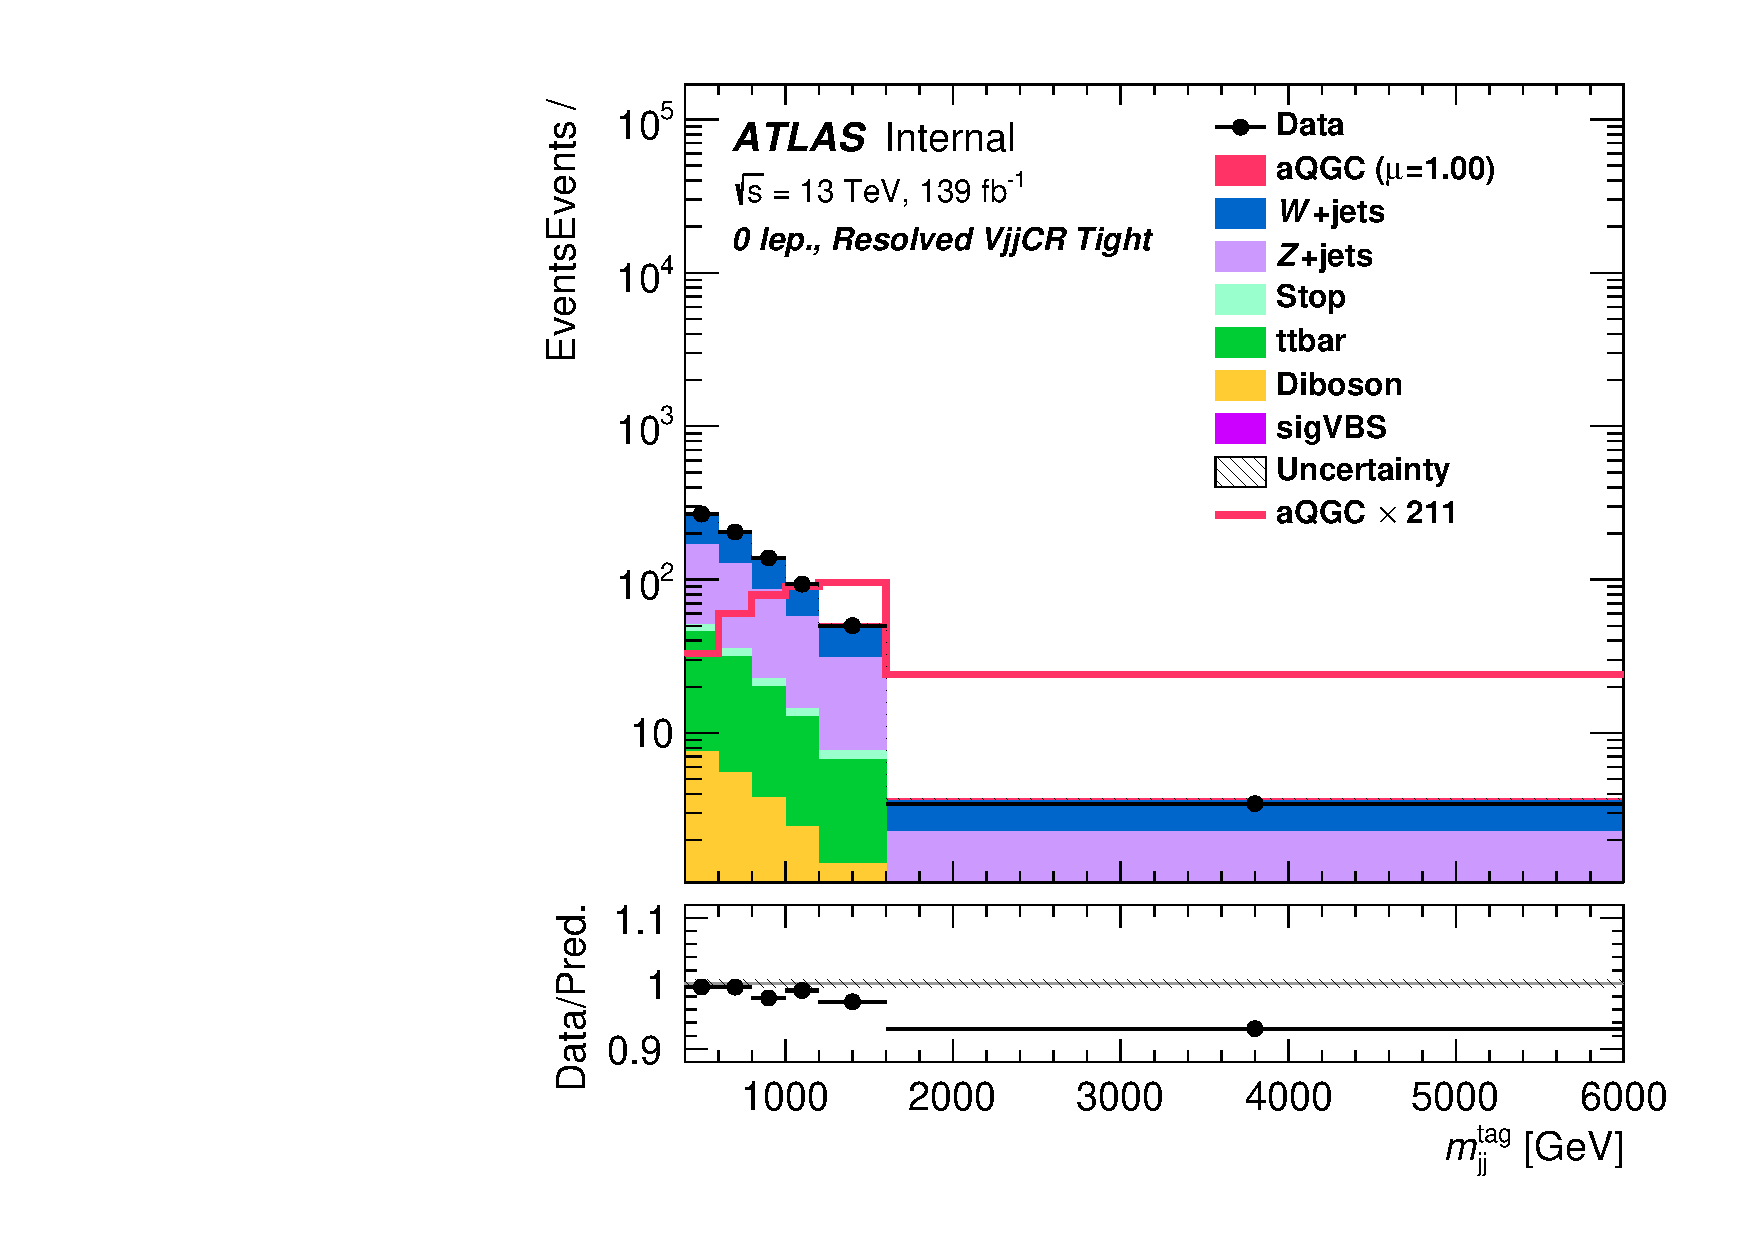
\includegraphics[width=0.32\textwidth]{figures/aQGC/Region_distMTagJets_DCRVjetFid_BMin0_T0_Y6051_incTag1_J2_L0_incJet1_Prefitlog.pdf}}
%    	\subfigure[ 2lep resolved SR ]{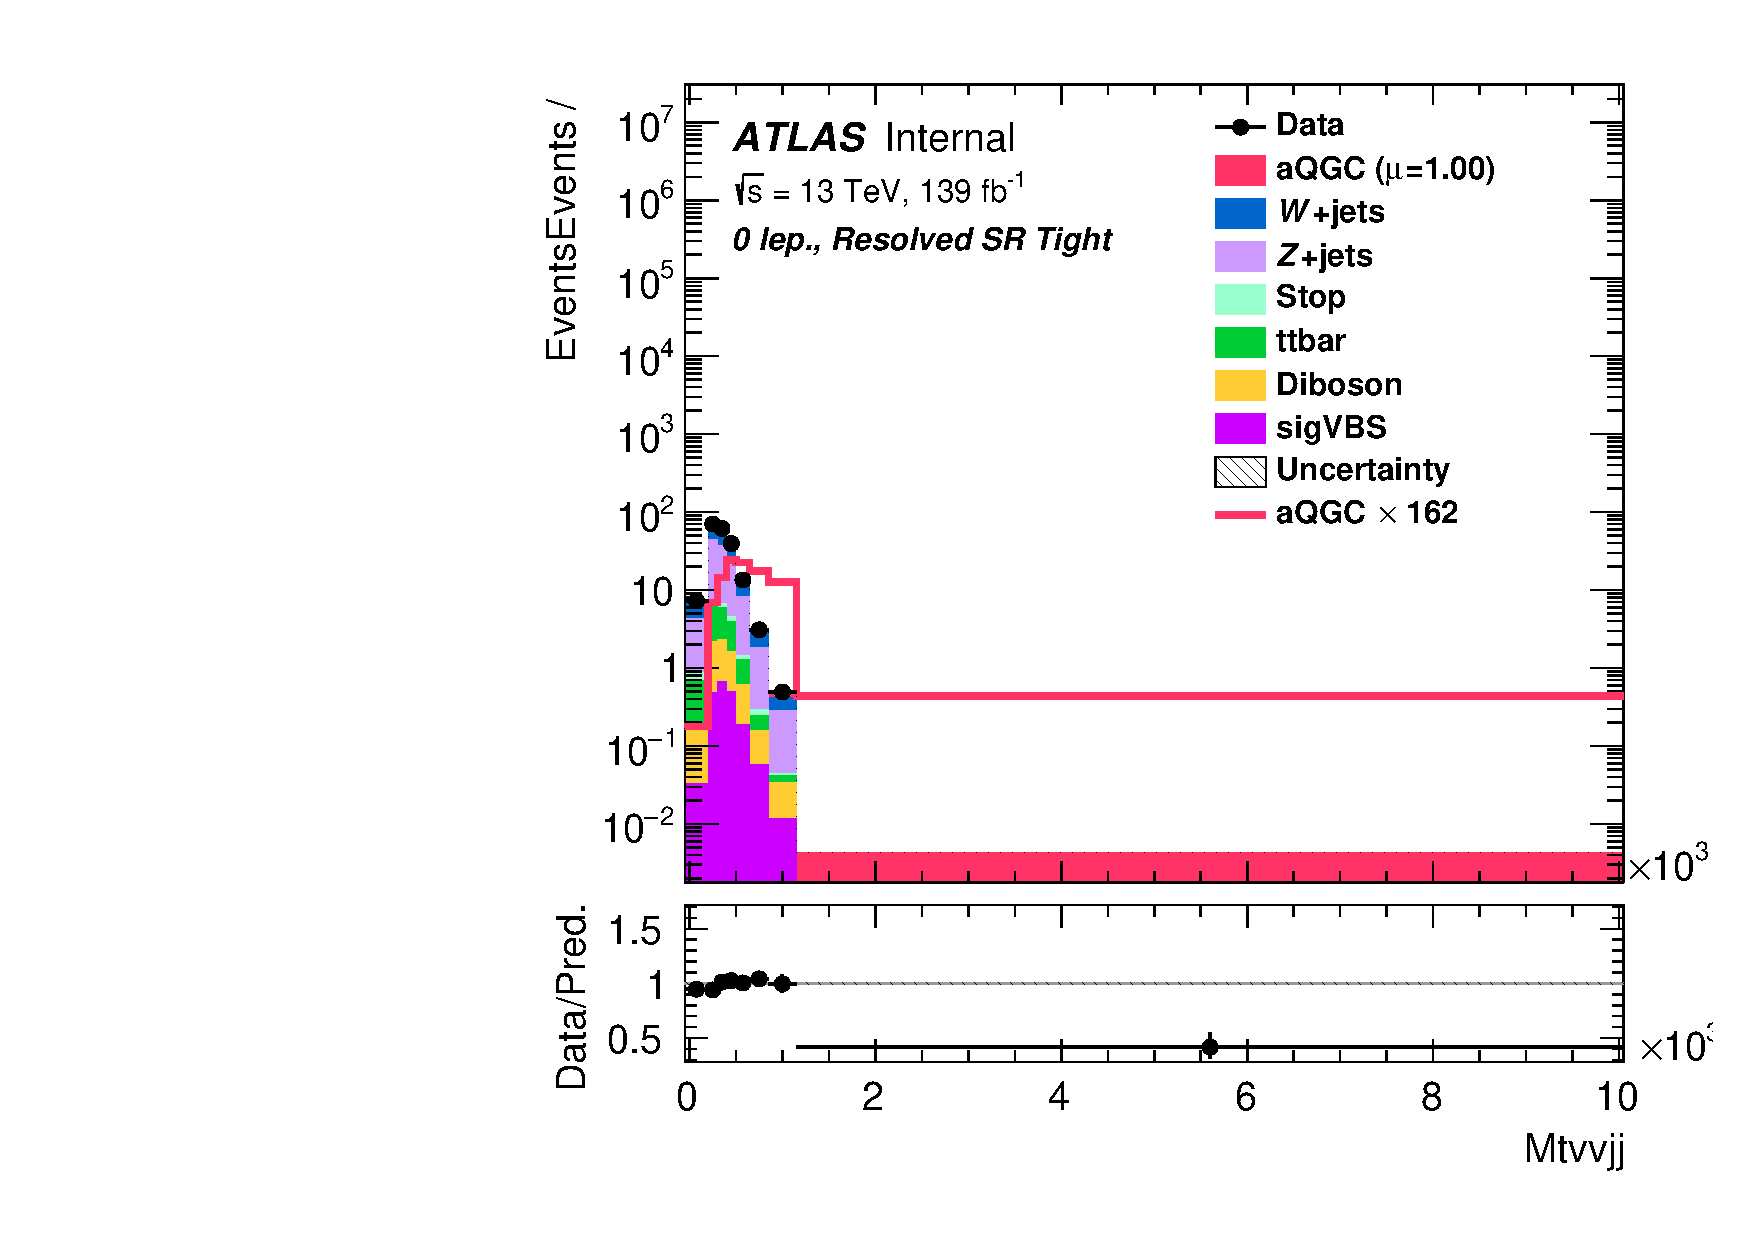
\includegraphics[width=0.32\textwidth]{figures/aQGC/Region_distMtvvjj_DSRVBSFid_BMin0_T0_Y6051_incTag1_J2_L0_incJet1_Prefitlog.pdf}}
%        \caption{Prefit plots for operator FT0 in \tlep channel are shown. The standard model EW signal is floated as the background.}
%        \label{fig:2lepFT0}
%\end{figure}
%
